\documentclass[titlepage]{article}

% Suppresses chktex warnings 
% chktex-file 1
% chktex-file 3
% chktex-file 8
% chktex-file 10
% chktex-file 17
% chktex-file 24
% chktex-file 26
% chktex-file 36
% chktex-file 44
% chktex-file 46

\usepackage{geometry}
\usepackage{tikz}
\usetikzlibrary{fit}
\usetikzlibrary{positioning}
\usetikzlibrary{intersections}
\usetikzlibrary{matrix}
\usepackage{pgf}        % Used to import pgf figures with \input
\def\mathdefault#1{#1}  % Fixes 'Undefined control sequence \mathdefault' in imported pgf files
\usepackage{pgfplots}
\usepgfplotslibrary{fillbetween}
\pgfplotsset{compat=1.18}
\pgfplotsset{hide xscale/.style={/pgfplots/xtick scale label code/.code={}}}
\pgfplotsset{hide yscale/.style={/pgfplots/ytick scale label code/.code={}}}
\usepackage{amsmath}
\usepackage{upgreek}
\usepackage{url}
\hyphenation{}	        % Correct bad hyphenation
\usepackage{graphicx}   % For including figures and pictures
\usepackage{float}      % Used to fix location of images i.e.\begin{figure}[H]
\usepackage{fancyhdr}   % For headers and footers
\pagestyle{fancy}
\usepackage{lastpage}   % Allows referencing last page (for footer)
\usepackage{listings}   % For highlighting code
\usepackage{titling}    % To reference title, author, and date
\usepackage{array}      % For fixed-width tables
\usepackage{makecell}   % Formats individual table cells
\usepackage{multirow}   % For multi-row columns (Top left justify header)
\usepackage[american]{circuitikz} % Used to draw circuit and block diagrams
\usepackage{appendix}   
\usepackage{xcolor}     % For coloring code listings
\usepackage{colortbl}   % For coloring table cells
\definecolor{nraoblue}{rgb}{0.776,0.851,0.945}  % Color of table headers
\usepackage{enumitem}   % For formatting enumerated lists
\usepackage[parfill]{parskip}               % Removes paragraph indentation, adds line break
\usepackage[hang, flushmargin]{footmisc}    % Removes footnote indentation
\setenumerate[1]{label={(\arabic*)}}
\usepackage[backend=biber,style=numeric,sorting=none]{biblatex}
\addbibresource{references.bib}
\usepackage{hyperref}   % Allows hyperlinks
\hypersetup{
  colorlinks   = true,  % Colors links instead of ugly boxes
  filecolor    = blue,  % Color for local hyperlinks
  linkcolor    = ., % Color for internal hyperlinks
  citecolor    = ., % Color for citations
  urlcolor     = blue,  % Color for linked urls
}
\usepackage{caption}    % Changes figure/table caption color and size
\definecolor{captioncolor}{RGB}{79,129,189}
\captionsetup{font={
    small, 
    color=captioncolor,
    bf,
}}
 

% Changes font from Computer Modern to Gill Sans MT
% This requires XeLaTeX or LuaTeX to function
% Add "latex-workshop.latex.recipe.default": "latexmk (xelatex)" to workspace.json
\usepackage{fontspec}
\setmainfont{gil.ttf}[
    BoldFont        = gil-b.ttf,
    ItalicFont      = gil-i.ttf,
    BoldItalicFont  = gil-bi.ttf,
]

% Code listing styling
\definecolor{codegreen}{rgb}{0,0.6,0}
\definecolor{codegray}{rgb}{0.5,0.5,0.5}
\definecolor{codepurple}{rgb}{0.58,0,0.82}
\definecolor{backcolour}{rgb}{0.95,0.95,0.92}

\lstdefinestyle{mystyle}{
    backgroundcolor=\color{backcolour},   
    commentstyle=\color{codegreen},
    keywordstyle=\color{magenta},
    numberstyle=\tiny\color{codegray},
    stringstyle=\color{codepurple},
    basicstyle=\ttfamily\footnotesize,
    breakatwhitespace=false,         
    breaklines=true,                 
    captionpos=b,                    
    keepspaces=true,                 
    numbers=left,                    
    numbersep=5pt,                  
    showspaces=false,                
    showstringspaces=false,
    showtabs=false,                  
    tabsize=2
}

\lstset{style=mystyle}
% Global TikZ parameters
\tikzset{every picture/.style={/utils/exec={\fontfamily{lmr}}}}
\ctikzset{sources/fill=red!20}
\ctikzset{chips/fill=cyan!20}
\ctikzset{electromechanicals/fill=blue!20}
\ctikzset{blocks/fill=green!20}
\ctikzset{amplifiers/fill=yellow!30}
\tikzset{amp/.append style={fill=yellow!30}}
\tikzset{twoport/.append style={fill=cyan!20}}
% TikZ node[server] symbol
\makeatletter
\pgfkeys{/pgf/.cd,
  parallelepiped offset x/.initial=2mm,
  parallelepiped offset y/.initial=2mm
}
\pgfdeclareshape{parallelepiped}
{
  \inheritsavedanchors[from=rectangle] % this is nearly a rectangle
  \inheritanchorborder[from=rectangle]
  \inheritanchor[from=rectangle]{north}
  \inheritanchor[from=rectangle]{north west}
  \inheritanchor[from=rectangle]{north east}
  \inheritanchor[from=rectangle]{center}
  \inheritanchor[from=rectangle]{west}
  \inheritanchor[from=rectangle]{east}
  \inheritanchor[from=rectangle]{mid}
  \inheritanchor[from=rectangle]{mid west}
  \inheritanchor[from=rectangle]{mid east}
  \inheritanchor[from=rectangle]{base}
  \inheritanchor[from=rectangle]{base west}
  \inheritanchor[from=rectangle]{base east}
  \inheritanchor[from=rectangle]{south}
  \inheritanchor[from=rectangle]{south west}
  \inheritanchor[from=rectangle]{south east}
  \backgroundpath{
    % store lower right in xa/ya and upper right in xb/yb
    \southwest \pgf@xa=\pgf@x \pgf@ya=\pgf@y
    \northeast \pgf@xb=\pgf@x \pgf@yb=\pgf@y
    \pgfmathsetlength\pgfutil@tempdima{\pgfkeysvalueof{/pgf/parallelepiped
      offset x}}
    \pgfmathsetlength\pgfutil@tempdimb{\pgfkeysvalueof{/pgf/parallelepiped
      offset y}}
    \def\ppd@offset{\pgfpoint{\pgfutil@tempdima}{\pgfutil@tempdimb}}
    \pgfpathmoveto{\pgfqpoint{\pgf@xa}{\pgf@ya}}
    \pgfpathlineto{\pgfqpoint{\pgf@xb}{\pgf@ya}}
    \pgfpathlineto{\pgfqpoint{\pgf@xb}{\pgf@yb}}
    \pgfpathlineto{\pgfqpoint{\pgf@xa}{\pgf@yb}}
    \pgfpathclose
    \pgfpathmoveto{\pgfqpoint{\pgf@xb}{\pgf@ya}}
    \pgfpathlineto{\pgfpointadd{\pgfpoint{\pgf@xb}{\pgf@ya}}{\ppd@offset}}
    \pgfpathlineto{\pgfpointadd{\pgfpoint{\pgf@xb}{\pgf@yb}}{\ppd@offset}}
    \pgfpathlineto{\pgfpointadd{\pgfpoint{\pgf@xa}{\pgf@yb}}{\ppd@offset}}
    \pgfpathlineto{\pgfqpoint{\pgf@xa}{\pgf@yb}}
    \pgfpathmoveto{\pgfqpoint{\pgf@xb}{\pgf@yb}}
    \pgfpathlineto{\pgfpointadd{\pgfpoint{\pgf@xb}{\pgf@yb}}{\ppd@offset}}
  }
}
\makeatother
% I don't even remember what this does
\tikzset{
  ports/.style={
    line width=0.3pt,
    top color=gray!20,
    bottom color=gray!80
  },
  server/.style={
    parallelepiped,
    fill=white, draw,
    minimum width=0.35cm,
    minimum height=0.75cm,
    parallelepiped offset x=3mm,
    parallelepiped offset y=2mm,
    xscale=-1,
    path picture={
      \draw[top color=gray!5,bottom color=gray!40]
      (path picture bounding box.south west) rectangle 
      (path picture bounding box.north east);
      \coordinate (A-center) at ($(path picture bounding box.center)!0!(path
        picture bounding box.south)$);
      \coordinate (A-west) at ([xshift=-0.575cm]path picture bounding box.west);
      \draw[ports]([yshift=0.1cm]$(A-west)!0!(A-center)$)
        rectangle +(0.2,0.065);
      \draw[ports]([yshift=0.01cm]$(A-west)!0.085!(A-center)$)
        rectangle +(0.15,0.05);
      \fill[black]([yshift=-0.35cm]$(A-west)!-0.1!(A-center)$)
        rectangle +(0.235,0.0175);
      \fill[black]([yshift=-0.385cm]$(A-west)!-0.1!(A-center)$)
        rectangle +(0.235,0.0175);
      \fill[black]([yshift=-0.42cm]$(A-west)!-0.1!(A-center)$)
        rectangle +(0.235,0.0175);
    }  
  },
}
% Adds key for current tikz coordinate
\newcommand\currentpos{\the\tikz@lastxsaved,\the\tikz@lastysaved}
% Wiring diagram matrix stuff (syntax for jumping lines and block styles)
\tikzset{
    connect/.style args={(#1) to (#2) over #3 by #4}{
        insert path={
            \pgfextra{
                \pgfinterruptpath
                    \path [name path=userpath] (#1) -- (#2);
                    \path [name intersections={of=userpath and #3,by=overpoint}];
                \endpgfinterruptpath                
            }
            let \p1=($(#1)-(overpoint)$), \n1={veclen(\x1,\y1)}, 
                            \n2={atan2(\y1,\x1)}, \n3={abs(#4)}, \n4={#4>0 ?180:-180}  in 
                            (#1) -- ($(#1)!\n1-\n3!(overpoint)$) 
                            arc (\n2:\n2+\n4:\n3) -- (#2)
        }
    },
}
\tikzset{wire board/.style={
          matrix of nodes,
          row sep={17pt, between origins},
          nodes={anchor=center, minimum height=14pt} % set min height or else distance from matrix.north to first row will change depending on the content of the first row
          },
        wiresright/.style={
          column 1/.style={nodes={left}},
          column 2/.style={font=\bfseries},
          column 3/.style={nodes={above right}},
          },
        wiresboth/.style={
          column 1/.style={nodes={above left}},
          column 2/.style={font=\bfseries},
          column 4/.style={font=\bfseries},
          column 5/.style={nodes={above right}},
          },
        wiresleft/.style={
          column 1/.style={nodes={above left}},
          column 2/.style={font=\bfseries},
          column 3/.style={nodes={right}},
        },
}

% The following lines define a new command \nraocite that cites references in NRAO format RD0X by redefining \cite command to remove brackets. \nraoprecite includes a prenote.
\DeclareCiteCommand{\cite} [\mkbibemph{\emph{}}]
  {\usebibmacro{prenote}}
  {\usebibmacro{citeindex}%
   \printtext[bibhyperref]{\usebibmacro{cite}}}
  {\multicitedelim}
  {\usebibmacro{postnote}}
\DeclareCiteCommand*{\cite} [\mkbibemph\emph{}]
  {\usebibmacro{prenote}}
  {\usebibmacro{citeindex}
   \printtext[bibhyperref]{\usebibmacro{citeyear}}}
  {\multicitedelim}
  {\usebibmacro{postnote}}
\newcommand{\nraocite}[1]{[RD0\cite{#1}]}
\newcommand{\nraoprecite}[2][]{[RD0\cite{#2}{, #1}]}


% ASSIGN TITLE, AUTHOR, DATE, DOCUMENT NUMBER, STATUS, HERE
\title{Title goes here}
\author{Author
    }% <-this % stops a space
\date{Jan 1, 2000}
\def\docnum{DOC NUM}
\def\status{\textcolor{red}{DRAFT}}

% HEADERS AND FOOTERS
\renewcommand{\headrulewidth}{0pt}
\fancyheadoffset[L,R]{2cm}
\fancyhead[L]{\vspace{-1cm}
\includegraphics[width=2cm]{images/NRAO Logo Badge.png}}
\fancyhead[R]{
\renewcommand{\arraystretch}{1.4}
\renewcommand{\arrayrulewidth}{0.25pt}
\begin{tabular}{|w{l}{6.7cm}|w{l}{4.9cm}|w{l}{3.4cm}|}
    \hline
        \multirow[t]{2}{6.7cm}{\textit{\textbf{Title:}} \thetitle} &
        \textit{\textbf{Owner:}} \theauthor &
        \textit{\textbf{Date:}}  \thedate \\
            &   &   \\
    \hline
        \multicolumn{2}{|l|}{
            \textit{\textbf{NRAO Doc \#:}} \docnum  
        } &
        \textit{\textbf{Version:}} A \\
    \hline
\end{tabular}
}
\fancyfoot[C]{Page \textbf{\thepage} of \textbf{\pageref{LastPage}}}

 % DOCUMENT STARTS HERE
\begin{document}
\setlength{\leftmargin}{1in}        % Sets margin
\setlength{\rightmargin}{1in}       % Sets margin
\setlength{\voffset}{-1.2in}        % Moves header up
\setlength{\headheight}{3.5cm}      % Defines header height
\setlength{\textheight}{591pt}      % Extends text/body size down
\setlength{\footskip}{60pt}         % Defines gap between body and footer

\thispagestyle{fancy}
\begin{center}
     
\includegraphics[width=5cm]{images/NRAO Logo Badge.png} \\
     \vspace*{0.5cm}
     \textbf{\huge\thetitle} \\
     \vspace*{0.5cm}
     \large\docnum \\
     \Large Status: \status \\
     \vspace*{0.6cm} \large
     % FIRST TABLE HERE
     \begin{tabular}{|m{6.93cm}|m{4.5cm}|m{2cm}|} \hline
        \rowcolor{nraoblue}
        \textbf{Prepared By} & \textbf{Organization} & \textbf{Date} \\ \hline
        \makecell[l]{Author\\Title} & NRAO Electronics Div. & 1/1/2000 \\ 
        \hline
    \end{tabular} \\
    \vspace*{0.8cm}
    \begin{tabular}{|m{3cm}|m{3.5cm}|m{6.93cm}|} \hline
        \rowcolor{nraoblue}
        \textbf{Approvals} & \textbf{Organization} & \textbf{Signatures} \\ \hline
    \end{tabular}
    \renewcommand{\arraystretch}{2}
    % CONTENT OF SECOND TABLE HERE
    \begin{tabular}{|w{l}{3cm}|m{3.5cm}|m{6.93cm}|} \hline
        \parbox{3cm}{\raggedright
        Name\\Title
        } & NRAO Electronics Division \raggedright &  \\ 
        \hline
        \parbox{3cm}{\raggedright
        Name\\Title
        } & NRAO Electronics Division \raggedright &  \\ 
        \hline
        \parbox{3cm}{\raggedright
        Name\\Title
        } & NRAO Electronics Division \raggedright &  \\ 
        \hline
    \end{tabular} \\
    \renewcommand{\arraystretch}{1}
    \vspace*{0.8cm}
    \begin{tabular}{|m{3cm}|m{3.5cm}|m{6.93cm}|} \hline
        \rowcolor{nraoblue}
        \textbf{Released By} & \textbf{Organization} & \textbf{Signature} \\ \hline
    \end{tabular}
    \renewcommand{\arraystretch}{1.5}
    % CONTENT OF THIRD TABLE HERE
    \begin{tabular}{|m{3cm}|m{3.5cm}|m{6.93cm}|} \hline
        \parbox{3cm}{\raggedright
        Name\\Title
        } & NRAO Electronics Division \raggedright &  \\ 
        \hline
    \end{tabular}
    \renewcommand{\arraystretch}{1}
\end{center}

% CHANGE RECORD
\newpage
\section*{Change Record}
\begin{center}
\renewcommand{\arraystretch}{1.2}
    \begin{tabular}{|m{1.5cm}|m{2.2cm}|m{2.5cm}|m{1.7cm}|m{5cm}|} \hline
        \rowcolor{nraoblue}
        Version & Date & Author & Affected\newline Section(s) & Reason\\ \hline
    \end{tabular}
\renewcommand{\arraystretch}{1.6}
    \begin{tabular}{|m{1.5cm}|m{2.2cm}|m{2.5cm}|m{1.7cm}|m{5cm}|} \hline
        01 & Aug 15, 2023 & R. Nguyen & All & Initial Draft \\ \hline
        02 & Aug 16, 2023 & \makecell[l]{T. Anderson\\R. Nguyen} & All & Edits \\ \hline
        A  & Aug 16, 2023 & T. Anderson & All & Review \\ \hline
          &          &           &     &               \\ \hline
          &          &           &     &               \\ \hline
          &          &           &     &               \\ \hline
          &          &           &     &               \\ \hline
    \end{tabular}
\renewcommand{\arraystretch}{1}
\end{center}

\newpage
\tableofcontents
\listoffigures
\thispagestyle{fancy}
\newpage

% DOCUMENT STARTS HERE
\section{Introduction}

\subsection{What is the RF-DFS and RF-EMS?}
copy from readme/wiki/plan or something

The Radio Frequency - Direction Finding System and Environmental Monitoring System are tools utilized by the NRAO-NM Interference Protection Group to identify and locate RF interference at the Very Large Array. The former is a 3-meter dish antenna with azimuth and elevation drives whereas the latter is a 50-foot tower with an omnidirectional club antenna. Both are connected to the RFI shack and controlled by a Python front end. This interface allows a user to control RF switching between both antennas and log data through a spectrum analyzer. 

\subsection{System Overview}
The three locations of note are the RFI shack, the RF-DFS dish, and the RF-EMS tower. A block diagram which shows the breakdown of major components and their connections is shown in Figure~\ref{fig:sysblock2}. The user will be able to control all IO functions through the Python application run on the PC (emsmonpc2).  SCPI commands issued over GPIB allow the user to control and view the spectrum analyzer display on the PC and a serial connection facilitates the same function with the motor controller. This motor controller is a Parker Hannifin ACR9000 which drives 2 Aries AR-04AE servos; one each for azimuth and elevation. RF switching is controlled by a PLC in the RFI shack (not shown).

\begin{figure}[!ht]
  \begin{center}
      \begin{circuitikz}
          % Shack
          \draw(0, 0) node[server, scale=1.5, name=computer]{};
          % \draw(computer.east) ++ (0.5, 0.2) node[anchor=west](computerlabel){PC};
          \draw(computer.west) node[anchor=east]{};
          \ctikzset{bipoles/oscope/waveform=triangle}
          \ctikzset{bipoles/oscope/width=1.0}
          \draw(computer.west)  ++ (-1, 0.2) 
          coordinate(ctrwest)-- ++ (-1.2, 0)
          node[oscopeshape, anchor=east](spec){};
          \draw(spec.west) -- ++ (-1.2, 0)
          node[twoportshape, anchor=east](shackswitch){};
          \draw(shackswitch.center) node[spdt, scale=0.6, xscale=-1]{};
          \draw(ctrwest) ++ (-0.6, 0) node[anchor=south]{GPIB};
          \draw(spec.south) node[anchor=north]{N9040b};
          \draw(spec.in 1) node[ocirc, scale=0.7]{};
          \draw(spec.in 2) node[ocirc, scale=0.7]{};
          \draw(spec.west) ++ (-0.6, 0) node[anchor=south]{Coax};

          % DFS
          \draw(shackswitch.west) -- ++ (-2, 0)
          to[amp, invert] ++ (-2, 0)
          to[amp, invert, name=dfslna1] ++ (-2, 0)
          -| ++ (-1, 0)
          coordinate(dfs)
          -- ++ (0, 0.5)
          node[bareantenna, anchor=south](dfsantenna){};
          % \draw(dfslna1.east) ++ (0.5, 0.5) node[anchor=south](){PMA3-14LN+};

          % EMS
          % \draw(spec.north) -- ++ (0, 1.5)
          % to[amp, invert, name=emslna2] ++ (0, 2)
          % to[amp, invert, name=emslna1] ++ (0, 2)
          % node[bareantenna, anchor=south](emsantenna){};
          \draw(shackswitch.north) -- ++ (0, 2)
          node[twoportshape, name=s1]{} -- ++ (0, 0.8)
          to[amp, boxed, invert] ++ (0, 1) -- ++ (0, 0.8)
          node[twoportshape, name=s2]{} -- ++ (0, 0.8)
          node[bareantenna, anchor=south](emsantenna){};
          % \draw(spec.north) ++ (0, 0.75) node[anchor=west]{Coax};
          \draw(s1.center) node[spdt, scale=0.6, rotate=90]{};
          \draw(s2.center) node[spdt, xscale=-1, scale=0.6, rotate=270]{};
          % \draw(emslna1) ++ (0, -0.7) node[anchor=west](emslnalabel){PMA3-14LN+};

          % Motor stuff
          \draw(computer.south) |- ++ (-8.5, -1)
          node[qfpchip, anchor=west, external pins width=0, hide numbers, name=acr, scale=0.8, align=center]{Motor\\Ctrl.};
          \draw(computer.south) ++ (0, -1)
          node[anchor=south east](seriallabel){RS-485};
          \draw([yshift=-8pt]acr.west) -- ++ (-2, 0)
          node[elmech, rotate=90, anchor=bottom](m2){};
          \draw(m2) [->, dashed] -| ([yshift=-10pt]dfs.center);
          \draw([yshift=8pt]acr.west) -- ++ (-0.6, 0)
          node[elmech, rotate=90, anchor=bottom](m1){};
          %\draw(m1) [->] -- ++ (3, 0) -- ([yshift=-10pt, xshift=-10pt]dfs.center);
          \path[name path = border3](dfs.center) -- ++ (0, -2);
          \path[name path = line3, overlay](m1.top) -- ++ (-5, 0);
          \draw[name intersections={of=border3 and line3}, dashed] (m1.top) -- (intersection-1)
          node[diamondpole]{};
          \draw(m1.center) node{Az};
          \draw(m2.center) node{El};

          % Boxes
          \node[draw, rectangle, dashed, fit=(dfsantenna) (acr), inner sep=10](dfsbox){};
          \node[draw, rectangle, dashed, fit=(emsantenna) (s1), inner sep=10](emsbox){};
          \node[draw, rectangle, dashed, fit=(shackswitch) (computer), inner sep=10](shackbox){};

          % Box Labels
          \draw(dfsbox.north) node[anchor=south]{RF - DFS};
          \draw(emsbox.west) node[anchor=east]{RF - EMS};
          \draw(shackbox.north east) node[anchor=south east]{RFI Shack};
      \end{circuitikz}
  \caption{System block diagram (not including PLC).}\label{fig:sysblock2}
  \end{center}
\end{figure}

\subsection{RF Signal Chain}
Each system has a single 50-10000 MHz receiver but the framework is in place to add additional receivers relatively easily. Figure~\ref{fig:rfblock} shows an RF block diagram of existing components and the plan for an additional 6-18 GHz receiver on the EMS tower.

All switches are Dynatech Microwave M4-413K201L SP4T relay switches. Switches S2 and S3 are already installed in the EMS tower to make adding a receiver as streamlined as possible. The reason there are no switches at the DFS is because it requires either a redesign of the LNA housing to fit relay switches or solid state switches that are integrated on a board with the other RF components.

The coaxial cables running up the tower and to the dish are Andrew LDF1-50 1/4'' heliax cables with an upper frequency limit of 15800 MHz. The loss is around 21 dB/100ft at 16 GHz, as such, it may be required to build a downconverting stage for any higher frequency receivers, especially with the relatively long cable runs present in these systems.

The LNAs in these initial 50-10000 MHz receivers are Mini-Circuits PMA3-14LN+ wideband low noise MMICs. The boards that house these amplifiers are designed in house and fabricated on OSHPark 4-layer stackups in order to save cost over using prebuilt components. Figure~\ref{fig:pma3} shows the gain and noise figure of an assembled amplifier over the operating frequency.

\begin{figure}[!ht]
    \begin{center}
        \begin{circuitikz}
            % \draw[help lines, dashed] grid (14, 3);
            % \draw[help lines, dashed] grid (14, -3);

            \draw(0, 0) node[bnc](port1){N9040b};
            \draw(port1.hot) -- ++ (1, 0)
            node[rotary switch = 4 in 60 wiper 60, anchor=in](sw1){};
            
            \draw(sw1.out 1) -- ++ (0.75, 0) 
            to[twoport, name=emscableloss, fill=green!20] ++ (0, 2.75)
            -- ++ (0.75, 0)
            node[rotary switch = 4 in 60 wiper 60, anchor=in](sw2){};
            \draw (emscableloss.center) node[resistorshape, anchor = center, rotate = 90, scale = 0.8]{};
            
            % EMS low band
            \draw(sw2.out 1) -| ++ (1, 0.5) coordinate(abcd)
            -- ++ (0.5, 0)
            to[amp, invert, t=\ctikzflipx{\footnotesize LNA}] ++ (2.75, 0)
            coordinate(emsref1)
            to[amp, invert, t=\ctikzflipx{\footnotesize LNA}] ++ (2.75, 0)
            -- ++ (0.5, 0)
            coordinate(p1);
            
            % EMS downconverted stage
            \draw(sw2.out 2) -- (current subpath start -| abcd)
            -- ++ (0, -0.75)
            coordinate(asdf)
            -- ++ (0.25 ,0)
            to[amp, invert, name=ifamp, t=\ctikzflipx{IF}] ++ (1.5, 0)
            -- ++ (0.25, 0) node[mixer, anchor=w, name=mixer1, fill=cyan!20]{};
            \draw(mixer1.e) -- ++ (0.25, 0)
            to[bandpass] ++ (1.5, 0)
            to[amp, invert, name=rfamp, t=\ctikzflipx{RF}] ++ (1.5, 0) -- ++ (0.25, 0)
            coordinate(p2);
            \draw(mixer1.s)[<-] -- ++ (0, -0.5)
            node[oscillator, anchor=north, fill=cyan!20](pll){LO};
            
            % DFS
            \draw(sw1.out 2) -| ++ (0.5, 0)
            to[twoport, name=dfscableloss, fill=green!20] (current subpath start -| asdf)
            -- (current subpath start -| p2)
            node[ampshape, xscale=-1, anchor=east, fill=yellow!30, t=\ctikzflipx{\footnotesize LNA}](dfsref1){};
            \draw(dfsref1.west)
            to[amp, invert, t=\ctikzflipx{\footnotesize LNA}] ++ (2, 0)
            node[bnc, xscale=-1](port3){\ctikzflipx{DFS}};
            \draw (dfscableloss.center) node[resistorshape, anchor = center, rotate = 90, scale = 0.8]{};
            
            % EMS port
            \draw(sw2 -| p1) ++ (1, 0)
            node[rotary switch = 4 in 60 wiper 60, xscale=-1](sw3){};
            \draw(sw3.out 1) -| (p1);
            \draw(sw3.out 2) -| (p2);
            \draw(sw3.in) -- (sw3.in -| port3)
            node[bnc, xscale=-1](port2){\ctikzflipx{EMS}};

            % Switch labels and arrows
            \draw(sw1.north) node[anchor=south](sw1lab){S1};
            \draw(sw2.north) node[anchor=south](sw2lab){S2};
            \draw(sw3.north) node[anchor=south](sw3lab){S3};
            \draw(sw1lab.north) [dashed, <-] -- ++ (0, 3.5) coordinate(sw1plclabel) node[anchor=south]{PLC};
            \draw(sw2lab.north) [dashed, <-] -- (sw2lab.north |- sw1plclabel) node[anchor=south]{PLC};
            \draw(sw3lab.north) [dashed, <-] -- (sw3lab.north |- sw1plclabel) node[anchor=south]{PLC};

            % Phase 3 box            
            \node[draw, rectangle, dashed, fit=(ifamp) (rfamp) (pll), inner sep=8](ph3box){};

            % Labels
            \draw([yshift=2pt]dfscableloss.north)[<-] -- ++ (0, 0.15) node[anchor=south](cablelosslabel){Cable loss};
            \draw(cablelosslabel.north)[->] to [bend right=45] ([xshift=2pt]emscableloss.south);
            \draw(ph3box.south east) node[anchor=south east]{Future Upgrade};
            % \draw(emsref1.north |- sw1plclabel) node[anchor=south]{PMA3-14LN+};
            % \draw(dfsref1.north) ++ (0.8, 0.2) node[anchor=south]{PMA3-14LN+};
        \end{circuitikz}
    \caption{Phase 2 Block Diagram}\label{fig:rfblock}
    \end{center}
\end{figure}
\begin{figure}[!ht]
  \begin{center}
    %% Creator: Matplotlib, PGF backend
%%
%% To include the figure in your LaTeX document, write
%%   \input{<filename>.pgf}
%%
%% Make sure the required packages are loaded in your preamble
%%   \usepackage{pgf}
%%
%% Also ensure that all the required font packages are loaded; for instance,
%% the lmodern package is sometimes necessary when using math font.
%%   \usepackage{lmodern}
%%
%% Figures using additional raster images can only be included by \input if
%% they are in the same directory as the main LaTeX file. For loading figures
%% from other directories you can use the `import` package
%%   \usepackage{import}
%%
%% and then include the figures with
%%   \import{<path to file>}{<filename>.pgf}
%%
%% Matplotlib used the following preamble
%%   \def\mathdefault#1{#1}
%%   \everymath=\expandafter{\the\everymath\displaystyle}
%%   
%%   \ifdefined\pdftexversion\else  % non-pdftex case.
%%     \usepackage{fontspec}
%%   \fi
%%   \makeatletter\@ifpackageloaded{underscore}{}{\usepackage[strings]{underscore}}\makeatother
%%
\begingroup%
\makeatletter%
\begin{pgfpicture}%
\pgfpathrectangle{\pgfpointorigin}{\pgfqpoint{4.800000in}{3.600000in}}%
\pgfusepath{use as bounding box, clip}%
\begin{pgfscope}%
\pgfsetbuttcap%
\pgfsetmiterjoin%
\definecolor{currentfill}{rgb}{1.000000,1.000000,1.000000}%
\pgfsetfillcolor{currentfill}%
\pgfsetlinewidth{0.000000pt}%
\definecolor{currentstroke}{rgb}{1.000000,1.000000,1.000000}%
\pgfsetstrokecolor{currentstroke}%
\pgfsetdash{}{0pt}%
\pgfpathmoveto{\pgfqpoint{0.000000in}{0.000000in}}%
\pgfpathlineto{\pgfqpoint{4.800000in}{0.000000in}}%
\pgfpathlineto{\pgfqpoint{4.800000in}{3.600000in}}%
\pgfpathlineto{\pgfqpoint{0.000000in}{3.600000in}}%
\pgfpathlineto{\pgfqpoint{0.000000in}{0.000000in}}%
\pgfpathclose%
\pgfusepath{fill}%
\end{pgfscope}%
\begin{pgfscope}%
\pgfsetbuttcap%
\pgfsetmiterjoin%
\definecolor{currentfill}{rgb}{1.000000,1.000000,1.000000}%
\pgfsetfillcolor{currentfill}%
\pgfsetlinewidth{0.000000pt}%
\definecolor{currentstroke}{rgb}{0.000000,0.000000,0.000000}%
\pgfsetstrokecolor{currentstroke}%
\pgfsetstrokeopacity{0.000000}%
\pgfsetdash{}{0pt}%
\pgfpathmoveto{\pgfqpoint{0.435417in}{0.423750in}}%
\pgfpathlineto{\pgfqpoint{4.416667in}{0.423750in}}%
\pgfpathlineto{\pgfqpoint{4.416667in}{3.338250in}}%
\pgfpathlineto{\pgfqpoint{0.435417in}{3.338250in}}%
\pgfpathlineto{\pgfqpoint{0.435417in}{0.423750in}}%
\pgfpathclose%
\pgfusepath{fill}%
\end{pgfscope}%
\begin{pgfscope}%
\pgfpathrectangle{\pgfqpoint{0.435417in}{0.423750in}}{\pgfqpoint{3.981250in}{2.914500in}}%
\pgfusepath{clip}%
\pgfsetrectcap%
\pgfsetroundjoin%
\pgfsetlinewidth{0.803000pt}%
\definecolor{currentstroke}{rgb}{0.690196,0.690196,0.690196}%
\pgfsetstrokecolor{currentstroke}%
\pgfsetdash{}{0pt}%
\pgfpathmoveto{\pgfqpoint{0.435417in}{0.423750in}}%
\pgfpathlineto{\pgfqpoint{0.435417in}{3.338250in}}%
\pgfusepath{stroke}%
\end{pgfscope}%
\begin{pgfscope}%
\pgfsetbuttcap%
\pgfsetroundjoin%
\definecolor{currentfill}{rgb}{0.000000,0.000000,0.000000}%
\pgfsetfillcolor{currentfill}%
\pgfsetlinewidth{0.803000pt}%
\definecolor{currentstroke}{rgb}{0.000000,0.000000,0.000000}%
\pgfsetstrokecolor{currentstroke}%
\pgfsetdash{}{0pt}%
\pgfsys@defobject{currentmarker}{\pgfqpoint{0.000000in}{-0.048611in}}{\pgfqpoint{0.000000in}{0.000000in}}{%
\pgfpathmoveto{\pgfqpoint{0.000000in}{0.000000in}}%
\pgfpathlineto{\pgfqpoint{0.000000in}{-0.048611in}}%
\pgfusepath{stroke,fill}%
}%
\begin{pgfscope}%
\pgfsys@transformshift{0.435417in}{0.423750in}%
\pgfsys@useobject{currentmarker}{}%
\end{pgfscope}%
\end{pgfscope}%
\begin{pgfscope}%
\definecolor{textcolor}{rgb}{0.000000,0.000000,0.000000}%
\pgfsetstrokecolor{textcolor}%
\pgfsetfillcolor{textcolor}%
\pgftext[x=0.435417in,y=0.326527in,,top]{\color{textcolor}{\rmfamily\fontsize{10.000000}{12.000000}\selectfont\catcode`\^=\active\def^{\ifmmode\sp\else\^{}\fi}\catcode`\%=\active\def%{\%}$\mathdefault{0}$}}%
\end{pgfscope}%
\begin{pgfscope}%
\pgfpathrectangle{\pgfqpoint{0.435417in}{0.423750in}}{\pgfqpoint{3.981250in}{2.914500in}}%
\pgfusepath{clip}%
\pgfsetrectcap%
\pgfsetroundjoin%
\pgfsetlinewidth{0.803000pt}%
\definecolor{currentstroke}{rgb}{0.690196,0.690196,0.690196}%
\pgfsetstrokecolor{currentstroke}%
\pgfsetdash{}{0pt}%
\pgfpathmoveto{\pgfqpoint{1.231667in}{0.423750in}}%
\pgfpathlineto{\pgfqpoint{1.231667in}{3.338250in}}%
\pgfusepath{stroke}%
\end{pgfscope}%
\begin{pgfscope}%
\pgfsetbuttcap%
\pgfsetroundjoin%
\definecolor{currentfill}{rgb}{0.000000,0.000000,0.000000}%
\pgfsetfillcolor{currentfill}%
\pgfsetlinewidth{0.803000pt}%
\definecolor{currentstroke}{rgb}{0.000000,0.000000,0.000000}%
\pgfsetstrokecolor{currentstroke}%
\pgfsetdash{}{0pt}%
\pgfsys@defobject{currentmarker}{\pgfqpoint{0.000000in}{-0.048611in}}{\pgfqpoint{0.000000in}{0.000000in}}{%
\pgfpathmoveto{\pgfqpoint{0.000000in}{0.000000in}}%
\pgfpathlineto{\pgfqpoint{0.000000in}{-0.048611in}}%
\pgfusepath{stroke,fill}%
}%
\begin{pgfscope}%
\pgfsys@transformshift{1.231667in}{0.423750in}%
\pgfsys@useobject{currentmarker}{}%
\end{pgfscope}%
\end{pgfscope}%
\begin{pgfscope}%
\definecolor{textcolor}{rgb}{0.000000,0.000000,0.000000}%
\pgfsetstrokecolor{textcolor}%
\pgfsetfillcolor{textcolor}%
\pgftext[x=1.231667in,y=0.326527in,,top]{\color{textcolor}{\rmfamily\fontsize{10.000000}{12.000000}\selectfont\catcode`\^=\active\def^{\ifmmode\sp\else\^{}\fi}\catcode`\%=\active\def%{\%}$\mathdefault{2000}$}}%
\end{pgfscope}%
\begin{pgfscope}%
\pgfpathrectangle{\pgfqpoint{0.435417in}{0.423750in}}{\pgfqpoint{3.981250in}{2.914500in}}%
\pgfusepath{clip}%
\pgfsetrectcap%
\pgfsetroundjoin%
\pgfsetlinewidth{0.803000pt}%
\definecolor{currentstroke}{rgb}{0.690196,0.690196,0.690196}%
\pgfsetstrokecolor{currentstroke}%
\pgfsetdash{}{0pt}%
\pgfpathmoveto{\pgfqpoint{2.027917in}{0.423750in}}%
\pgfpathlineto{\pgfqpoint{2.027917in}{3.338250in}}%
\pgfusepath{stroke}%
\end{pgfscope}%
\begin{pgfscope}%
\pgfsetbuttcap%
\pgfsetroundjoin%
\definecolor{currentfill}{rgb}{0.000000,0.000000,0.000000}%
\pgfsetfillcolor{currentfill}%
\pgfsetlinewidth{0.803000pt}%
\definecolor{currentstroke}{rgb}{0.000000,0.000000,0.000000}%
\pgfsetstrokecolor{currentstroke}%
\pgfsetdash{}{0pt}%
\pgfsys@defobject{currentmarker}{\pgfqpoint{0.000000in}{-0.048611in}}{\pgfqpoint{0.000000in}{0.000000in}}{%
\pgfpathmoveto{\pgfqpoint{0.000000in}{0.000000in}}%
\pgfpathlineto{\pgfqpoint{0.000000in}{-0.048611in}}%
\pgfusepath{stroke,fill}%
}%
\begin{pgfscope}%
\pgfsys@transformshift{2.027917in}{0.423750in}%
\pgfsys@useobject{currentmarker}{}%
\end{pgfscope}%
\end{pgfscope}%
\begin{pgfscope}%
\definecolor{textcolor}{rgb}{0.000000,0.000000,0.000000}%
\pgfsetstrokecolor{textcolor}%
\pgfsetfillcolor{textcolor}%
\pgftext[x=2.027917in,y=0.326527in,,top]{\color{textcolor}{\rmfamily\fontsize{10.000000}{12.000000}\selectfont\catcode`\^=\active\def^{\ifmmode\sp\else\^{}\fi}\catcode`\%=\active\def%{\%}$\mathdefault{4000}$}}%
\end{pgfscope}%
\begin{pgfscope}%
\pgfpathrectangle{\pgfqpoint{0.435417in}{0.423750in}}{\pgfqpoint{3.981250in}{2.914500in}}%
\pgfusepath{clip}%
\pgfsetrectcap%
\pgfsetroundjoin%
\pgfsetlinewidth{0.803000pt}%
\definecolor{currentstroke}{rgb}{0.690196,0.690196,0.690196}%
\pgfsetstrokecolor{currentstroke}%
\pgfsetdash{}{0pt}%
\pgfpathmoveto{\pgfqpoint{2.824167in}{0.423750in}}%
\pgfpathlineto{\pgfqpoint{2.824167in}{3.338250in}}%
\pgfusepath{stroke}%
\end{pgfscope}%
\begin{pgfscope}%
\pgfsetbuttcap%
\pgfsetroundjoin%
\definecolor{currentfill}{rgb}{0.000000,0.000000,0.000000}%
\pgfsetfillcolor{currentfill}%
\pgfsetlinewidth{0.803000pt}%
\definecolor{currentstroke}{rgb}{0.000000,0.000000,0.000000}%
\pgfsetstrokecolor{currentstroke}%
\pgfsetdash{}{0pt}%
\pgfsys@defobject{currentmarker}{\pgfqpoint{0.000000in}{-0.048611in}}{\pgfqpoint{0.000000in}{0.000000in}}{%
\pgfpathmoveto{\pgfqpoint{0.000000in}{0.000000in}}%
\pgfpathlineto{\pgfqpoint{0.000000in}{-0.048611in}}%
\pgfusepath{stroke,fill}%
}%
\begin{pgfscope}%
\pgfsys@transformshift{2.824167in}{0.423750in}%
\pgfsys@useobject{currentmarker}{}%
\end{pgfscope}%
\end{pgfscope}%
\begin{pgfscope}%
\definecolor{textcolor}{rgb}{0.000000,0.000000,0.000000}%
\pgfsetstrokecolor{textcolor}%
\pgfsetfillcolor{textcolor}%
\pgftext[x=2.824167in,y=0.326527in,,top]{\color{textcolor}{\rmfamily\fontsize{10.000000}{12.000000}\selectfont\catcode`\^=\active\def^{\ifmmode\sp\else\^{}\fi}\catcode`\%=\active\def%{\%}$\mathdefault{6000}$}}%
\end{pgfscope}%
\begin{pgfscope}%
\pgfpathrectangle{\pgfqpoint{0.435417in}{0.423750in}}{\pgfqpoint{3.981250in}{2.914500in}}%
\pgfusepath{clip}%
\pgfsetrectcap%
\pgfsetroundjoin%
\pgfsetlinewidth{0.803000pt}%
\definecolor{currentstroke}{rgb}{0.690196,0.690196,0.690196}%
\pgfsetstrokecolor{currentstroke}%
\pgfsetdash{}{0pt}%
\pgfpathmoveto{\pgfqpoint{3.620417in}{0.423750in}}%
\pgfpathlineto{\pgfqpoint{3.620417in}{3.338250in}}%
\pgfusepath{stroke}%
\end{pgfscope}%
\begin{pgfscope}%
\pgfsetbuttcap%
\pgfsetroundjoin%
\definecolor{currentfill}{rgb}{0.000000,0.000000,0.000000}%
\pgfsetfillcolor{currentfill}%
\pgfsetlinewidth{0.803000pt}%
\definecolor{currentstroke}{rgb}{0.000000,0.000000,0.000000}%
\pgfsetstrokecolor{currentstroke}%
\pgfsetdash{}{0pt}%
\pgfsys@defobject{currentmarker}{\pgfqpoint{0.000000in}{-0.048611in}}{\pgfqpoint{0.000000in}{0.000000in}}{%
\pgfpathmoveto{\pgfqpoint{0.000000in}{0.000000in}}%
\pgfpathlineto{\pgfqpoint{0.000000in}{-0.048611in}}%
\pgfusepath{stroke,fill}%
}%
\begin{pgfscope}%
\pgfsys@transformshift{3.620417in}{0.423750in}%
\pgfsys@useobject{currentmarker}{}%
\end{pgfscope}%
\end{pgfscope}%
\begin{pgfscope}%
\definecolor{textcolor}{rgb}{0.000000,0.000000,0.000000}%
\pgfsetstrokecolor{textcolor}%
\pgfsetfillcolor{textcolor}%
\pgftext[x=3.620417in,y=0.326527in,,top]{\color{textcolor}{\rmfamily\fontsize{10.000000}{12.000000}\selectfont\catcode`\^=\active\def^{\ifmmode\sp\else\^{}\fi}\catcode`\%=\active\def%{\%}$\mathdefault{8000}$}}%
\end{pgfscope}%
\begin{pgfscope}%
\pgfpathrectangle{\pgfqpoint{0.435417in}{0.423750in}}{\pgfqpoint{3.981250in}{2.914500in}}%
\pgfusepath{clip}%
\pgfsetrectcap%
\pgfsetroundjoin%
\pgfsetlinewidth{0.803000pt}%
\definecolor{currentstroke}{rgb}{0.690196,0.690196,0.690196}%
\pgfsetstrokecolor{currentstroke}%
\pgfsetdash{}{0pt}%
\pgfpathmoveto{\pgfqpoint{4.416667in}{0.423750in}}%
\pgfpathlineto{\pgfqpoint{4.416667in}{3.338250in}}%
\pgfusepath{stroke}%
\end{pgfscope}%
\begin{pgfscope}%
\pgfsetbuttcap%
\pgfsetroundjoin%
\definecolor{currentfill}{rgb}{0.000000,0.000000,0.000000}%
\pgfsetfillcolor{currentfill}%
\pgfsetlinewidth{0.803000pt}%
\definecolor{currentstroke}{rgb}{0.000000,0.000000,0.000000}%
\pgfsetstrokecolor{currentstroke}%
\pgfsetdash{}{0pt}%
\pgfsys@defobject{currentmarker}{\pgfqpoint{0.000000in}{-0.048611in}}{\pgfqpoint{0.000000in}{0.000000in}}{%
\pgfpathmoveto{\pgfqpoint{0.000000in}{0.000000in}}%
\pgfpathlineto{\pgfqpoint{0.000000in}{-0.048611in}}%
\pgfusepath{stroke,fill}%
}%
\begin{pgfscope}%
\pgfsys@transformshift{4.416667in}{0.423750in}%
\pgfsys@useobject{currentmarker}{}%
\end{pgfscope}%
\end{pgfscope}%
\begin{pgfscope}%
\definecolor{textcolor}{rgb}{0.000000,0.000000,0.000000}%
\pgfsetstrokecolor{textcolor}%
\pgfsetfillcolor{textcolor}%
\pgftext[x=4.416667in,y=0.326527in,,top]{\color{textcolor}{\rmfamily\fontsize{10.000000}{12.000000}\selectfont\catcode`\^=\active\def^{\ifmmode\sp\else\^{}\fi}\catcode`\%=\active\def%{\%}$\mathdefault{10000}$}}%
\end{pgfscope}%
\begin{pgfscope}%
\pgfsetbuttcap%
\pgfsetroundjoin%
\definecolor{currentfill}{rgb}{0.000000,0.000000,0.000000}%
\pgfsetfillcolor{currentfill}%
\pgfsetlinewidth{0.602250pt}%
\definecolor{currentstroke}{rgb}{0.000000,0.000000,0.000000}%
\pgfsetstrokecolor{currentstroke}%
\pgfsetdash{}{0pt}%
\pgfsys@defobject{currentmarker}{\pgfqpoint{0.000000in}{-0.027778in}}{\pgfqpoint{0.000000in}{0.000000in}}{%
\pgfpathmoveto{\pgfqpoint{0.000000in}{0.000000in}}%
\pgfpathlineto{\pgfqpoint{0.000000in}{-0.027778in}}%
\pgfusepath{stroke,fill}%
}%
\begin{pgfscope}%
\pgfsys@transformshift{0.634479in}{0.423750in}%
\pgfsys@useobject{currentmarker}{}%
\end{pgfscope}%
\end{pgfscope}%
\begin{pgfscope}%
\pgfsetbuttcap%
\pgfsetroundjoin%
\definecolor{currentfill}{rgb}{0.000000,0.000000,0.000000}%
\pgfsetfillcolor{currentfill}%
\pgfsetlinewidth{0.602250pt}%
\definecolor{currentstroke}{rgb}{0.000000,0.000000,0.000000}%
\pgfsetstrokecolor{currentstroke}%
\pgfsetdash{}{0pt}%
\pgfsys@defobject{currentmarker}{\pgfqpoint{0.000000in}{-0.027778in}}{\pgfqpoint{0.000000in}{0.000000in}}{%
\pgfpathmoveto{\pgfqpoint{0.000000in}{0.000000in}}%
\pgfpathlineto{\pgfqpoint{0.000000in}{-0.027778in}}%
\pgfusepath{stroke,fill}%
}%
\begin{pgfscope}%
\pgfsys@transformshift{0.833542in}{0.423750in}%
\pgfsys@useobject{currentmarker}{}%
\end{pgfscope}%
\end{pgfscope}%
\begin{pgfscope}%
\pgfsetbuttcap%
\pgfsetroundjoin%
\definecolor{currentfill}{rgb}{0.000000,0.000000,0.000000}%
\pgfsetfillcolor{currentfill}%
\pgfsetlinewidth{0.602250pt}%
\definecolor{currentstroke}{rgb}{0.000000,0.000000,0.000000}%
\pgfsetstrokecolor{currentstroke}%
\pgfsetdash{}{0pt}%
\pgfsys@defobject{currentmarker}{\pgfqpoint{0.000000in}{-0.027778in}}{\pgfqpoint{0.000000in}{0.000000in}}{%
\pgfpathmoveto{\pgfqpoint{0.000000in}{0.000000in}}%
\pgfpathlineto{\pgfqpoint{0.000000in}{-0.027778in}}%
\pgfusepath{stroke,fill}%
}%
\begin{pgfscope}%
\pgfsys@transformshift{1.032604in}{0.423750in}%
\pgfsys@useobject{currentmarker}{}%
\end{pgfscope}%
\end{pgfscope}%
\begin{pgfscope}%
\pgfsetbuttcap%
\pgfsetroundjoin%
\definecolor{currentfill}{rgb}{0.000000,0.000000,0.000000}%
\pgfsetfillcolor{currentfill}%
\pgfsetlinewidth{0.602250pt}%
\definecolor{currentstroke}{rgb}{0.000000,0.000000,0.000000}%
\pgfsetstrokecolor{currentstroke}%
\pgfsetdash{}{0pt}%
\pgfsys@defobject{currentmarker}{\pgfqpoint{0.000000in}{-0.027778in}}{\pgfqpoint{0.000000in}{0.000000in}}{%
\pgfpathmoveto{\pgfqpoint{0.000000in}{0.000000in}}%
\pgfpathlineto{\pgfqpoint{0.000000in}{-0.027778in}}%
\pgfusepath{stroke,fill}%
}%
\begin{pgfscope}%
\pgfsys@transformshift{1.430729in}{0.423750in}%
\pgfsys@useobject{currentmarker}{}%
\end{pgfscope}%
\end{pgfscope}%
\begin{pgfscope}%
\pgfsetbuttcap%
\pgfsetroundjoin%
\definecolor{currentfill}{rgb}{0.000000,0.000000,0.000000}%
\pgfsetfillcolor{currentfill}%
\pgfsetlinewidth{0.602250pt}%
\definecolor{currentstroke}{rgb}{0.000000,0.000000,0.000000}%
\pgfsetstrokecolor{currentstroke}%
\pgfsetdash{}{0pt}%
\pgfsys@defobject{currentmarker}{\pgfqpoint{0.000000in}{-0.027778in}}{\pgfqpoint{0.000000in}{0.000000in}}{%
\pgfpathmoveto{\pgfqpoint{0.000000in}{0.000000in}}%
\pgfpathlineto{\pgfqpoint{0.000000in}{-0.027778in}}%
\pgfusepath{stroke,fill}%
}%
\begin{pgfscope}%
\pgfsys@transformshift{1.629792in}{0.423750in}%
\pgfsys@useobject{currentmarker}{}%
\end{pgfscope}%
\end{pgfscope}%
\begin{pgfscope}%
\pgfsetbuttcap%
\pgfsetroundjoin%
\definecolor{currentfill}{rgb}{0.000000,0.000000,0.000000}%
\pgfsetfillcolor{currentfill}%
\pgfsetlinewidth{0.602250pt}%
\definecolor{currentstroke}{rgb}{0.000000,0.000000,0.000000}%
\pgfsetstrokecolor{currentstroke}%
\pgfsetdash{}{0pt}%
\pgfsys@defobject{currentmarker}{\pgfqpoint{0.000000in}{-0.027778in}}{\pgfqpoint{0.000000in}{0.000000in}}{%
\pgfpathmoveto{\pgfqpoint{0.000000in}{0.000000in}}%
\pgfpathlineto{\pgfqpoint{0.000000in}{-0.027778in}}%
\pgfusepath{stroke,fill}%
}%
\begin{pgfscope}%
\pgfsys@transformshift{1.828854in}{0.423750in}%
\pgfsys@useobject{currentmarker}{}%
\end{pgfscope}%
\end{pgfscope}%
\begin{pgfscope}%
\pgfsetbuttcap%
\pgfsetroundjoin%
\definecolor{currentfill}{rgb}{0.000000,0.000000,0.000000}%
\pgfsetfillcolor{currentfill}%
\pgfsetlinewidth{0.602250pt}%
\definecolor{currentstroke}{rgb}{0.000000,0.000000,0.000000}%
\pgfsetstrokecolor{currentstroke}%
\pgfsetdash{}{0pt}%
\pgfsys@defobject{currentmarker}{\pgfqpoint{0.000000in}{-0.027778in}}{\pgfqpoint{0.000000in}{0.000000in}}{%
\pgfpathmoveto{\pgfqpoint{0.000000in}{0.000000in}}%
\pgfpathlineto{\pgfqpoint{0.000000in}{-0.027778in}}%
\pgfusepath{stroke,fill}%
}%
\begin{pgfscope}%
\pgfsys@transformshift{2.226979in}{0.423750in}%
\pgfsys@useobject{currentmarker}{}%
\end{pgfscope}%
\end{pgfscope}%
\begin{pgfscope}%
\pgfsetbuttcap%
\pgfsetroundjoin%
\definecolor{currentfill}{rgb}{0.000000,0.000000,0.000000}%
\pgfsetfillcolor{currentfill}%
\pgfsetlinewidth{0.602250pt}%
\definecolor{currentstroke}{rgb}{0.000000,0.000000,0.000000}%
\pgfsetstrokecolor{currentstroke}%
\pgfsetdash{}{0pt}%
\pgfsys@defobject{currentmarker}{\pgfqpoint{0.000000in}{-0.027778in}}{\pgfqpoint{0.000000in}{0.000000in}}{%
\pgfpathmoveto{\pgfqpoint{0.000000in}{0.000000in}}%
\pgfpathlineto{\pgfqpoint{0.000000in}{-0.027778in}}%
\pgfusepath{stroke,fill}%
}%
\begin{pgfscope}%
\pgfsys@transformshift{2.426042in}{0.423750in}%
\pgfsys@useobject{currentmarker}{}%
\end{pgfscope}%
\end{pgfscope}%
\begin{pgfscope}%
\pgfsetbuttcap%
\pgfsetroundjoin%
\definecolor{currentfill}{rgb}{0.000000,0.000000,0.000000}%
\pgfsetfillcolor{currentfill}%
\pgfsetlinewidth{0.602250pt}%
\definecolor{currentstroke}{rgb}{0.000000,0.000000,0.000000}%
\pgfsetstrokecolor{currentstroke}%
\pgfsetdash{}{0pt}%
\pgfsys@defobject{currentmarker}{\pgfqpoint{0.000000in}{-0.027778in}}{\pgfqpoint{0.000000in}{0.000000in}}{%
\pgfpathmoveto{\pgfqpoint{0.000000in}{0.000000in}}%
\pgfpathlineto{\pgfqpoint{0.000000in}{-0.027778in}}%
\pgfusepath{stroke,fill}%
}%
\begin{pgfscope}%
\pgfsys@transformshift{2.625104in}{0.423750in}%
\pgfsys@useobject{currentmarker}{}%
\end{pgfscope}%
\end{pgfscope}%
\begin{pgfscope}%
\pgfsetbuttcap%
\pgfsetroundjoin%
\definecolor{currentfill}{rgb}{0.000000,0.000000,0.000000}%
\pgfsetfillcolor{currentfill}%
\pgfsetlinewidth{0.602250pt}%
\definecolor{currentstroke}{rgb}{0.000000,0.000000,0.000000}%
\pgfsetstrokecolor{currentstroke}%
\pgfsetdash{}{0pt}%
\pgfsys@defobject{currentmarker}{\pgfqpoint{0.000000in}{-0.027778in}}{\pgfqpoint{0.000000in}{0.000000in}}{%
\pgfpathmoveto{\pgfqpoint{0.000000in}{0.000000in}}%
\pgfpathlineto{\pgfqpoint{0.000000in}{-0.027778in}}%
\pgfusepath{stroke,fill}%
}%
\begin{pgfscope}%
\pgfsys@transformshift{3.023229in}{0.423750in}%
\pgfsys@useobject{currentmarker}{}%
\end{pgfscope}%
\end{pgfscope}%
\begin{pgfscope}%
\pgfsetbuttcap%
\pgfsetroundjoin%
\definecolor{currentfill}{rgb}{0.000000,0.000000,0.000000}%
\pgfsetfillcolor{currentfill}%
\pgfsetlinewidth{0.602250pt}%
\definecolor{currentstroke}{rgb}{0.000000,0.000000,0.000000}%
\pgfsetstrokecolor{currentstroke}%
\pgfsetdash{}{0pt}%
\pgfsys@defobject{currentmarker}{\pgfqpoint{0.000000in}{-0.027778in}}{\pgfqpoint{0.000000in}{0.000000in}}{%
\pgfpathmoveto{\pgfqpoint{0.000000in}{0.000000in}}%
\pgfpathlineto{\pgfqpoint{0.000000in}{-0.027778in}}%
\pgfusepath{stroke,fill}%
}%
\begin{pgfscope}%
\pgfsys@transformshift{3.222292in}{0.423750in}%
\pgfsys@useobject{currentmarker}{}%
\end{pgfscope}%
\end{pgfscope}%
\begin{pgfscope}%
\pgfsetbuttcap%
\pgfsetroundjoin%
\definecolor{currentfill}{rgb}{0.000000,0.000000,0.000000}%
\pgfsetfillcolor{currentfill}%
\pgfsetlinewidth{0.602250pt}%
\definecolor{currentstroke}{rgb}{0.000000,0.000000,0.000000}%
\pgfsetstrokecolor{currentstroke}%
\pgfsetdash{}{0pt}%
\pgfsys@defobject{currentmarker}{\pgfqpoint{0.000000in}{-0.027778in}}{\pgfqpoint{0.000000in}{0.000000in}}{%
\pgfpathmoveto{\pgfqpoint{0.000000in}{0.000000in}}%
\pgfpathlineto{\pgfqpoint{0.000000in}{-0.027778in}}%
\pgfusepath{stroke,fill}%
}%
\begin{pgfscope}%
\pgfsys@transformshift{3.421354in}{0.423750in}%
\pgfsys@useobject{currentmarker}{}%
\end{pgfscope}%
\end{pgfscope}%
\begin{pgfscope}%
\pgfsetbuttcap%
\pgfsetroundjoin%
\definecolor{currentfill}{rgb}{0.000000,0.000000,0.000000}%
\pgfsetfillcolor{currentfill}%
\pgfsetlinewidth{0.602250pt}%
\definecolor{currentstroke}{rgb}{0.000000,0.000000,0.000000}%
\pgfsetstrokecolor{currentstroke}%
\pgfsetdash{}{0pt}%
\pgfsys@defobject{currentmarker}{\pgfqpoint{0.000000in}{-0.027778in}}{\pgfqpoint{0.000000in}{0.000000in}}{%
\pgfpathmoveto{\pgfqpoint{0.000000in}{0.000000in}}%
\pgfpathlineto{\pgfqpoint{0.000000in}{-0.027778in}}%
\pgfusepath{stroke,fill}%
}%
\begin{pgfscope}%
\pgfsys@transformshift{3.819479in}{0.423750in}%
\pgfsys@useobject{currentmarker}{}%
\end{pgfscope}%
\end{pgfscope}%
\begin{pgfscope}%
\pgfsetbuttcap%
\pgfsetroundjoin%
\definecolor{currentfill}{rgb}{0.000000,0.000000,0.000000}%
\pgfsetfillcolor{currentfill}%
\pgfsetlinewidth{0.602250pt}%
\definecolor{currentstroke}{rgb}{0.000000,0.000000,0.000000}%
\pgfsetstrokecolor{currentstroke}%
\pgfsetdash{}{0pt}%
\pgfsys@defobject{currentmarker}{\pgfqpoint{0.000000in}{-0.027778in}}{\pgfqpoint{0.000000in}{0.000000in}}{%
\pgfpathmoveto{\pgfqpoint{0.000000in}{0.000000in}}%
\pgfpathlineto{\pgfqpoint{0.000000in}{-0.027778in}}%
\pgfusepath{stroke,fill}%
}%
\begin{pgfscope}%
\pgfsys@transformshift{4.018542in}{0.423750in}%
\pgfsys@useobject{currentmarker}{}%
\end{pgfscope}%
\end{pgfscope}%
\begin{pgfscope}%
\pgfsetbuttcap%
\pgfsetroundjoin%
\definecolor{currentfill}{rgb}{0.000000,0.000000,0.000000}%
\pgfsetfillcolor{currentfill}%
\pgfsetlinewidth{0.602250pt}%
\definecolor{currentstroke}{rgb}{0.000000,0.000000,0.000000}%
\pgfsetstrokecolor{currentstroke}%
\pgfsetdash{}{0pt}%
\pgfsys@defobject{currentmarker}{\pgfqpoint{0.000000in}{-0.027778in}}{\pgfqpoint{0.000000in}{0.000000in}}{%
\pgfpathmoveto{\pgfqpoint{0.000000in}{0.000000in}}%
\pgfpathlineto{\pgfqpoint{0.000000in}{-0.027778in}}%
\pgfusepath{stroke,fill}%
}%
\begin{pgfscope}%
\pgfsys@transformshift{4.217604in}{0.423750in}%
\pgfsys@useobject{currentmarker}{}%
\end{pgfscope}%
\end{pgfscope}%
\begin{pgfscope}%
\definecolor{textcolor}{rgb}{0.000000,0.000000,0.000000}%
\pgfsetstrokecolor{textcolor}%
\pgfsetfillcolor{textcolor}%
\pgftext[x=2.426042in,y=0.147639in,,top]{\color{textcolor}{\rmfamily\fontsize{10.000000}{12.000000}\selectfont\catcode`\^=\active\def^{\ifmmode\sp\else\^{}\fi}\catcode`\%=\active\def%{\%}Frequency (MHz)}}%
\end{pgfscope}%
\begin{pgfscope}%
\pgfpathrectangle{\pgfqpoint{0.435417in}{0.423750in}}{\pgfqpoint{3.981250in}{2.914500in}}%
\pgfusepath{clip}%
\pgfsetrectcap%
\pgfsetroundjoin%
\pgfsetlinewidth{0.803000pt}%
\definecolor{currentstroke}{rgb}{0.690196,0.690196,0.690196}%
\pgfsetstrokecolor{currentstroke}%
\pgfsetdash{}{0pt}%
\pgfpathmoveto{\pgfqpoint{0.435417in}{0.423750in}}%
\pgfpathlineto{\pgfqpoint{4.416667in}{0.423750in}}%
\pgfusepath{stroke}%
\end{pgfscope}%
\begin{pgfscope}%
\pgfsetbuttcap%
\pgfsetroundjoin%
\definecolor{currentfill}{rgb}{0.000000,0.000000,0.000000}%
\pgfsetfillcolor{currentfill}%
\pgfsetlinewidth{0.803000pt}%
\definecolor{currentstroke}{rgb}{0.000000,0.000000,0.000000}%
\pgfsetstrokecolor{currentstroke}%
\pgfsetdash{}{0pt}%
\pgfsys@defobject{currentmarker}{\pgfqpoint{-0.048611in}{0.000000in}}{\pgfqpoint{-0.000000in}{0.000000in}}{%
\pgfpathmoveto{\pgfqpoint{-0.000000in}{0.000000in}}%
\pgfpathlineto{\pgfqpoint{-0.048611in}{0.000000in}}%
\pgfusepath{stroke,fill}%
}%
\begin{pgfscope}%
\pgfsys@transformshift{0.435417in}{0.423750in}%
\pgfsys@useobject{currentmarker}{}%
\end{pgfscope}%
\end{pgfscope}%
\begin{pgfscope}%
\definecolor{textcolor}{rgb}{0.000000,0.000000,1.000000}%
\pgfsetstrokecolor{textcolor}%
\pgfsetfillcolor{textcolor}%
\pgftext[x=0.268750in, y=0.375555in, left, base]{\color{textcolor}{\rmfamily\fontsize{10.000000}{12.000000}\selectfont\catcode`\^=\active\def^{\ifmmode\sp\else\^{}\fi}\catcode`\%=\active\def%{\%}$\mathdefault{0}$}}%
\end{pgfscope}%
\begin{pgfscope}%
\pgfpathrectangle{\pgfqpoint{0.435417in}{0.423750in}}{\pgfqpoint{3.981250in}{2.914500in}}%
\pgfusepath{clip}%
\pgfsetrectcap%
\pgfsetroundjoin%
\pgfsetlinewidth{0.803000pt}%
\definecolor{currentstroke}{rgb}{0.690196,0.690196,0.690196}%
\pgfsetstrokecolor{currentstroke}%
\pgfsetdash{}{0pt}%
\pgfpathmoveto{\pgfqpoint{0.435417in}{1.006650in}}%
\pgfpathlineto{\pgfqpoint{4.416667in}{1.006650in}}%
\pgfusepath{stroke}%
\end{pgfscope}%
\begin{pgfscope}%
\pgfsetbuttcap%
\pgfsetroundjoin%
\definecolor{currentfill}{rgb}{0.000000,0.000000,0.000000}%
\pgfsetfillcolor{currentfill}%
\pgfsetlinewidth{0.803000pt}%
\definecolor{currentstroke}{rgb}{0.000000,0.000000,0.000000}%
\pgfsetstrokecolor{currentstroke}%
\pgfsetdash{}{0pt}%
\pgfsys@defobject{currentmarker}{\pgfqpoint{-0.048611in}{0.000000in}}{\pgfqpoint{-0.000000in}{0.000000in}}{%
\pgfpathmoveto{\pgfqpoint{-0.000000in}{0.000000in}}%
\pgfpathlineto{\pgfqpoint{-0.048611in}{0.000000in}}%
\pgfusepath{stroke,fill}%
}%
\begin{pgfscope}%
\pgfsys@transformshift{0.435417in}{1.006650in}%
\pgfsys@useobject{currentmarker}{}%
\end{pgfscope}%
\end{pgfscope}%
\begin{pgfscope}%
\definecolor{textcolor}{rgb}{0.000000,0.000000,1.000000}%
\pgfsetstrokecolor{textcolor}%
\pgfsetfillcolor{textcolor}%
\pgftext[x=0.268750in, y=0.958455in, left, base]{\color{textcolor}{\rmfamily\fontsize{10.000000}{12.000000}\selectfont\catcode`\^=\active\def^{\ifmmode\sp\else\^{}\fi}\catcode`\%=\active\def%{\%}$\mathdefault{5}$}}%
\end{pgfscope}%
\begin{pgfscope}%
\pgfpathrectangle{\pgfqpoint{0.435417in}{0.423750in}}{\pgfqpoint{3.981250in}{2.914500in}}%
\pgfusepath{clip}%
\pgfsetrectcap%
\pgfsetroundjoin%
\pgfsetlinewidth{0.803000pt}%
\definecolor{currentstroke}{rgb}{0.690196,0.690196,0.690196}%
\pgfsetstrokecolor{currentstroke}%
\pgfsetdash{}{0pt}%
\pgfpathmoveto{\pgfqpoint{0.435417in}{1.589550in}}%
\pgfpathlineto{\pgfqpoint{4.416667in}{1.589550in}}%
\pgfusepath{stroke}%
\end{pgfscope}%
\begin{pgfscope}%
\pgfsetbuttcap%
\pgfsetroundjoin%
\definecolor{currentfill}{rgb}{0.000000,0.000000,0.000000}%
\pgfsetfillcolor{currentfill}%
\pgfsetlinewidth{0.803000pt}%
\definecolor{currentstroke}{rgb}{0.000000,0.000000,0.000000}%
\pgfsetstrokecolor{currentstroke}%
\pgfsetdash{}{0pt}%
\pgfsys@defobject{currentmarker}{\pgfqpoint{-0.048611in}{0.000000in}}{\pgfqpoint{-0.000000in}{0.000000in}}{%
\pgfpathmoveto{\pgfqpoint{-0.000000in}{0.000000in}}%
\pgfpathlineto{\pgfqpoint{-0.048611in}{0.000000in}}%
\pgfusepath{stroke,fill}%
}%
\begin{pgfscope}%
\pgfsys@transformshift{0.435417in}{1.589550in}%
\pgfsys@useobject{currentmarker}{}%
\end{pgfscope}%
\end{pgfscope}%
\begin{pgfscope}%
\definecolor{textcolor}{rgb}{0.000000,0.000000,1.000000}%
\pgfsetstrokecolor{textcolor}%
\pgfsetfillcolor{textcolor}%
\pgftext[x=0.199305in, y=1.541355in, left, base]{\color{textcolor}{\rmfamily\fontsize{10.000000}{12.000000}\selectfont\catcode`\^=\active\def^{\ifmmode\sp\else\^{}\fi}\catcode`\%=\active\def%{\%}$\mathdefault{10}$}}%
\end{pgfscope}%
\begin{pgfscope}%
\pgfpathrectangle{\pgfqpoint{0.435417in}{0.423750in}}{\pgfqpoint{3.981250in}{2.914500in}}%
\pgfusepath{clip}%
\pgfsetrectcap%
\pgfsetroundjoin%
\pgfsetlinewidth{0.803000pt}%
\definecolor{currentstroke}{rgb}{0.690196,0.690196,0.690196}%
\pgfsetstrokecolor{currentstroke}%
\pgfsetdash{}{0pt}%
\pgfpathmoveto{\pgfqpoint{0.435417in}{2.172450in}}%
\pgfpathlineto{\pgfqpoint{4.416667in}{2.172450in}}%
\pgfusepath{stroke}%
\end{pgfscope}%
\begin{pgfscope}%
\pgfsetbuttcap%
\pgfsetroundjoin%
\definecolor{currentfill}{rgb}{0.000000,0.000000,0.000000}%
\pgfsetfillcolor{currentfill}%
\pgfsetlinewidth{0.803000pt}%
\definecolor{currentstroke}{rgb}{0.000000,0.000000,0.000000}%
\pgfsetstrokecolor{currentstroke}%
\pgfsetdash{}{0pt}%
\pgfsys@defobject{currentmarker}{\pgfqpoint{-0.048611in}{0.000000in}}{\pgfqpoint{-0.000000in}{0.000000in}}{%
\pgfpathmoveto{\pgfqpoint{-0.000000in}{0.000000in}}%
\pgfpathlineto{\pgfqpoint{-0.048611in}{0.000000in}}%
\pgfusepath{stroke,fill}%
}%
\begin{pgfscope}%
\pgfsys@transformshift{0.435417in}{2.172450in}%
\pgfsys@useobject{currentmarker}{}%
\end{pgfscope}%
\end{pgfscope}%
\begin{pgfscope}%
\definecolor{textcolor}{rgb}{0.000000,0.000000,1.000000}%
\pgfsetstrokecolor{textcolor}%
\pgfsetfillcolor{textcolor}%
\pgftext[x=0.199305in, y=2.124255in, left, base]{\color{textcolor}{\rmfamily\fontsize{10.000000}{12.000000}\selectfont\catcode`\^=\active\def^{\ifmmode\sp\else\^{}\fi}\catcode`\%=\active\def%{\%}$\mathdefault{15}$}}%
\end{pgfscope}%
\begin{pgfscope}%
\pgfpathrectangle{\pgfqpoint{0.435417in}{0.423750in}}{\pgfqpoint{3.981250in}{2.914500in}}%
\pgfusepath{clip}%
\pgfsetrectcap%
\pgfsetroundjoin%
\pgfsetlinewidth{0.803000pt}%
\definecolor{currentstroke}{rgb}{0.690196,0.690196,0.690196}%
\pgfsetstrokecolor{currentstroke}%
\pgfsetdash{}{0pt}%
\pgfpathmoveto{\pgfqpoint{0.435417in}{2.755350in}}%
\pgfpathlineto{\pgfqpoint{4.416667in}{2.755350in}}%
\pgfusepath{stroke}%
\end{pgfscope}%
\begin{pgfscope}%
\pgfsetbuttcap%
\pgfsetroundjoin%
\definecolor{currentfill}{rgb}{0.000000,0.000000,0.000000}%
\pgfsetfillcolor{currentfill}%
\pgfsetlinewidth{0.803000pt}%
\definecolor{currentstroke}{rgb}{0.000000,0.000000,0.000000}%
\pgfsetstrokecolor{currentstroke}%
\pgfsetdash{}{0pt}%
\pgfsys@defobject{currentmarker}{\pgfqpoint{-0.048611in}{0.000000in}}{\pgfqpoint{-0.000000in}{0.000000in}}{%
\pgfpathmoveto{\pgfqpoint{-0.000000in}{0.000000in}}%
\pgfpathlineto{\pgfqpoint{-0.048611in}{0.000000in}}%
\pgfusepath{stroke,fill}%
}%
\begin{pgfscope}%
\pgfsys@transformshift{0.435417in}{2.755350in}%
\pgfsys@useobject{currentmarker}{}%
\end{pgfscope}%
\end{pgfscope}%
\begin{pgfscope}%
\definecolor{textcolor}{rgb}{0.000000,0.000000,1.000000}%
\pgfsetstrokecolor{textcolor}%
\pgfsetfillcolor{textcolor}%
\pgftext[x=0.199305in, y=2.707155in, left, base]{\color{textcolor}{\rmfamily\fontsize{10.000000}{12.000000}\selectfont\catcode`\^=\active\def^{\ifmmode\sp\else\^{}\fi}\catcode`\%=\active\def%{\%}$\mathdefault{20}$}}%
\end{pgfscope}%
\begin{pgfscope}%
\pgfpathrectangle{\pgfqpoint{0.435417in}{0.423750in}}{\pgfqpoint{3.981250in}{2.914500in}}%
\pgfusepath{clip}%
\pgfsetrectcap%
\pgfsetroundjoin%
\pgfsetlinewidth{0.803000pt}%
\definecolor{currentstroke}{rgb}{0.690196,0.690196,0.690196}%
\pgfsetstrokecolor{currentstroke}%
\pgfsetdash{}{0pt}%
\pgfpathmoveto{\pgfqpoint{0.435417in}{3.338250in}}%
\pgfpathlineto{\pgfqpoint{4.416667in}{3.338250in}}%
\pgfusepath{stroke}%
\end{pgfscope}%
\begin{pgfscope}%
\pgfsetbuttcap%
\pgfsetroundjoin%
\definecolor{currentfill}{rgb}{0.000000,0.000000,0.000000}%
\pgfsetfillcolor{currentfill}%
\pgfsetlinewidth{0.803000pt}%
\definecolor{currentstroke}{rgb}{0.000000,0.000000,0.000000}%
\pgfsetstrokecolor{currentstroke}%
\pgfsetdash{}{0pt}%
\pgfsys@defobject{currentmarker}{\pgfqpoint{-0.048611in}{0.000000in}}{\pgfqpoint{-0.000000in}{0.000000in}}{%
\pgfpathmoveto{\pgfqpoint{-0.000000in}{0.000000in}}%
\pgfpathlineto{\pgfqpoint{-0.048611in}{0.000000in}}%
\pgfusepath{stroke,fill}%
}%
\begin{pgfscope}%
\pgfsys@transformshift{0.435417in}{3.338250in}%
\pgfsys@useobject{currentmarker}{}%
\end{pgfscope}%
\end{pgfscope}%
\begin{pgfscope}%
\definecolor{textcolor}{rgb}{0.000000,0.000000,1.000000}%
\pgfsetstrokecolor{textcolor}%
\pgfsetfillcolor{textcolor}%
\pgftext[x=0.199305in, y=3.290056in, left, base]{\color{textcolor}{\rmfamily\fontsize{10.000000}{12.000000}\selectfont\catcode`\^=\active\def^{\ifmmode\sp\else\^{}\fi}\catcode`\%=\active\def%{\%}$\mathdefault{25}$}}%
\end{pgfscope}%
\begin{pgfscope}%
\pgfsetbuttcap%
\pgfsetroundjoin%
\definecolor{currentfill}{rgb}{0.000000,0.000000,0.000000}%
\pgfsetfillcolor{currentfill}%
\pgfsetlinewidth{0.602250pt}%
\definecolor{currentstroke}{rgb}{0.000000,0.000000,0.000000}%
\pgfsetstrokecolor{currentstroke}%
\pgfsetdash{}{0pt}%
\pgfsys@defobject{currentmarker}{\pgfqpoint{-0.027778in}{0.000000in}}{\pgfqpoint{-0.000000in}{0.000000in}}{%
\pgfpathmoveto{\pgfqpoint{-0.000000in}{0.000000in}}%
\pgfpathlineto{\pgfqpoint{-0.027778in}{0.000000in}}%
\pgfusepath{stroke,fill}%
}%
\begin{pgfscope}%
\pgfsys@transformshift{0.435417in}{0.540330in}%
\pgfsys@useobject{currentmarker}{}%
\end{pgfscope}%
\end{pgfscope}%
\begin{pgfscope}%
\pgfsetbuttcap%
\pgfsetroundjoin%
\definecolor{currentfill}{rgb}{0.000000,0.000000,0.000000}%
\pgfsetfillcolor{currentfill}%
\pgfsetlinewidth{0.602250pt}%
\definecolor{currentstroke}{rgb}{0.000000,0.000000,0.000000}%
\pgfsetstrokecolor{currentstroke}%
\pgfsetdash{}{0pt}%
\pgfsys@defobject{currentmarker}{\pgfqpoint{-0.027778in}{0.000000in}}{\pgfqpoint{-0.000000in}{0.000000in}}{%
\pgfpathmoveto{\pgfqpoint{-0.000000in}{0.000000in}}%
\pgfpathlineto{\pgfqpoint{-0.027778in}{0.000000in}}%
\pgfusepath{stroke,fill}%
}%
\begin{pgfscope}%
\pgfsys@transformshift{0.435417in}{0.656910in}%
\pgfsys@useobject{currentmarker}{}%
\end{pgfscope}%
\end{pgfscope}%
\begin{pgfscope}%
\pgfsetbuttcap%
\pgfsetroundjoin%
\definecolor{currentfill}{rgb}{0.000000,0.000000,0.000000}%
\pgfsetfillcolor{currentfill}%
\pgfsetlinewidth{0.602250pt}%
\definecolor{currentstroke}{rgb}{0.000000,0.000000,0.000000}%
\pgfsetstrokecolor{currentstroke}%
\pgfsetdash{}{0pt}%
\pgfsys@defobject{currentmarker}{\pgfqpoint{-0.027778in}{0.000000in}}{\pgfqpoint{-0.000000in}{0.000000in}}{%
\pgfpathmoveto{\pgfqpoint{-0.000000in}{0.000000in}}%
\pgfpathlineto{\pgfqpoint{-0.027778in}{0.000000in}}%
\pgfusepath{stroke,fill}%
}%
\begin{pgfscope}%
\pgfsys@transformshift{0.435417in}{0.773490in}%
\pgfsys@useobject{currentmarker}{}%
\end{pgfscope}%
\end{pgfscope}%
\begin{pgfscope}%
\pgfsetbuttcap%
\pgfsetroundjoin%
\definecolor{currentfill}{rgb}{0.000000,0.000000,0.000000}%
\pgfsetfillcolor{currentfill}%
\pgfsetlinewidth{0.602250pt}%
\definecolor{currentstroke}{rgb}{0.000000,0.000000,0.000000}%
\pgfsetstrokecolor{currentstroke}%
\pgfsetdash{}{0pt}%
\pgfsys@defobject{currentmarker}{\pgfqpoint{-0.027778in}{0.000000in}}{\pgfqpoint{-0.000000in}{0.000000in}}{%
\pgfpathmoveto{\pgfqpoint{-0.000000in}{0.000000in}}%
\pgfpathlineto{\pgfqpoint{-0.027778in}{0.000000in}}%
\pgfusepath{stroke,fill}%
}%
\begin{pgfscope}%
\pgfsys@transformshift{0.435417in}{0.890070in}%
\pgfsys@useobject{currentmarker}{}%
\end{pgfscope}%
\end{pgfscope}%
\begin{pgfscope}%
\pgfsetbuttcap%
\pgfsetroundjoin%
\definecolor{currentfill}{rgb}{0.000000,0.000000,0.000000}%
\pgfsetfillcolor{currentfill}%
\pgfsetlinewidth{0.602250pt}%
\definecolor{currentstroke}{rgb}{0.000000,0.000000,0.000000}%
\pgfsetstrokecolor{currentstroke}%
\pgfsetdash{}{0pt}%
\pgfsys@defobject{currentmarker}{\pgfqpoint{-0.027778in}{0.000000in}}{\pgfqpoint{-0.000000in}{0.000000in}}{%
\pgfpathmoveto{\pgfqpoint{-0.000000in}{0.000000in}}%
\pgfpathlineto{\pgfqpoint{-0.027778in}{0.000000in}}%
\pgfusepath{stroke,fill}%
}%
\begin{pgfscope}%
\pgfsys@transformshift{0.435417in}{1.123230in}%
\pgfsys@useobject{currentmarker}{}%
\end{pgfscope}%
\end{pgfscope}%
\begin{pgfscope}%
\pgfsetbuttcap%
\pgfsetroundjoin%
\definecolor{currentfill}{rgb}{0.000000,0.000000,0.000000}%
\pgfsetfillcolor{currentfill}%
\pgfsetlinewidth{0.602250pt}%
\definecolor{currentstroke}{rgb}{0.000000,0.000000,0.000000}%
\pgfsetstrokecolor{currentstroke}%
\pgfsetdash{}{0pt}%
\pgfsys@defobject{currentmarker}{\pgfqpoint{-0.027778in}{0.000000in}}{\pgfqpoint{-0.000000in}{0.000000in}}{%
\pgfpathmoveto{\pgfqpoint{-0.000000in}{0.000000in}}%
\pgfpathlineto{\pgfqpoint{-0.027778in}{0.000000in}}%
\pgfusepath{stroke,fill}%
}%
\begin{pgfscope}%
\pgfsys@transformshift{0.435417in}{1.239810in}%
\pgfsys@useobject{currentmarker}{}%
\end{pgfscope}%
\end{pgfscope}%
\begin{pgfscope}%
\pgfsetbuttcap%
\pgfsetroundjoin%
\definecolor{currentfill}{rgb}{0.000000,0.000000,0.000000}%
\pgfsetfillcolor{currentfill}%
\pgfsetlinewidth{0.602250pt}%
\definecolor{currentstroke}{rgb}{0.000000,0.000000,0.000000}%
\pgfsetstrokecolor{currentstroke}%
\pgfsetdash{}{0pt}%
\pgfsys@defobject{currentmarker}{\pgfqpoint{-0.027778in}{0.000000in}}{\pgfqpoint{-0.000000in}{0.000000in}}{%
\pgfpathmoveto{\pgfqpoint{-0.000000in}{0.000000in}}%
\pgfpathlineto{\pgfqpoint{-0.027778in}{0.000000in}}%
\pgfusepath{stroke,fill}%
}%
\begin{pgfscope}%
\pgfsys@transformshift{0.435417in}{1.356390in}%
\pgfsys@useobject{currentmarker}{}%
\end{pgfscope}%
\end{pgfscope}%
\begin{pgfscope}%
\pgfsetbuttcap%
\pgfsetroundjoin%
\definecolor{currentfill}{rgb}{0.000000,0.000000,0.000000}%
\pgfsetfillcolor{currentfill}%
\pgfsetlinewidth{0.602250pt}%
\definecolor{currentstroke}{rgb}{0.000000,0.000000,0.000000}%
\pgfsetstrokecolor{currentstroke}%
\pgfsetdash{}{0pt}%
\pgfsys@defobject{currentmarker}{\pgfqpoint{-0.027778in}{0.000000in}}{\pgfqpoint{-0.000000in}{0.000000in}}{%
\pgfpathmoveto{\pgfqpoint{-0.000000in}{0.000000in}}%
\pgfpathlineto{\pgfqpoint{-0.027778in}{0.000000in}}%
\pgfusepath{stroke,fill}%
}%
\begin{pgfscope}%
\pgfsys@transformshift{0.435417in}{1.472970in}%
\pgfsys@useobject{currentmarker}{}%
\end{pgfscope}%
\end{pgfscope}%
\begin{pgfscope}%
\pgfsetbuttcap%
\pgfsetroundjoin%
\definecolor{currentfill}{rgb}{0.000000,0.000000,0.000000}%
\pgfsetfillcolor{currentfill}%
\pgfsetlinewidth{0.602250pt}%
\definecolor{currentstroke}{rgb}{0.000000,0.000000,0.000000}%
\pgfsetstrokecolor{currentstroke}%
\pgfsetdash{}{0pt}%
\pgfsys@defobject{currentmarker}{\pgfqpoint{-0.027778in}{0.000000in}}{\pgfqpoint{-0.000000in}{0.000000in}}{%
\pgfpathmoveto{\pgfqpoint{-0.000000in}{0.000000in}}%
\pgfpathlineto{\pgfqpoint{-0.027778in}{0.000000in}}%
\pgfusepath{stroke,fill}%
}%
\begin{pgfscope}%
\pgfsys@transformshift{0.435417in}{1.706130in}%
\pgfsys@useobject{currentmarker}{}%
\end{pgfscope}%
\end{pgfscope}%
\begin{pgfscope}%
\pgfsetbuttcap%
\pgfsetroundjoin%
\definecolor{currentfill}{rgb}{0.000000,0.000000,0.000000}%
\pgfsetfillcolor{currentfill}%
\pgfsetlinewidth{0.602250pt}%
\definecolor{currentstroke}{rgb}{0.000000,0.000000,0.000000}%
\pgfsetstrokecolor{currentstroke}%
\pgfsetdash{}{0pt}%
\pgfsys@defobject{currentmarker}{\pgfqpoint{-0.027778in}{0.000000in}}{\pgfqpoint{-0.000000in}{0.000000in}}{%
\pgfpathmoveto{\pgfqpoint{-0.000000in}{0.000000in}}%
\pgfpathlineto{\pgfqpoint{-0.027778in}{0.000000in}}%
\pgfusepath{stroke,fill}%
}%
\begin{pgfscope}%
\pgfsys@transformshift{0.435417in}{1.822710in}%
\pgfsys@useobject{currentmarker}{}%
\end{pgfscope}%
\end{pgfscope}%
\begin{pgfscope}%
\pgfsetbuttcap%
\pgfsetroundjoin%
\definecolor{currentfill}{rgb}{0.000000,0.000000,0.000000}%
\pgfsetfillcolor{currentfill}%
\pgfsetlinewidth{0.602250pt}%
\definecolor{currentstroke}{rgb}{0.000000,0.000000,0.000000}%
\pgfsetstrokecolor{currentstroke}%
\pgfsetdash{}{0pt}%
\pgfsys@defobject{currentmarker}{\pgfqpoint{-0.027778in}{0.000000in}}{\pgfqpoint{-0.000000in}{0.000000in}}{%
\pgfpathmoveto{\pgfqpoint{-0.000000in}{0.000000in}}%
\pgfpathlineto{\pgfqpoint{-0.027778in}{0.000000in}}%
\pgfusepath{stroke,fill}%
}%
\begin{pgfscope}%
\pgfsys@transformshift{0.435417in}{1.939290in}%
\pgfsys@useobject{currentmarker}{}%
\end{pgfscope}%
\end{pgfscope}%
\begin{pgfscope}%
\pgfsetbuttcap%
\pgfsetroundjoin%
\definecolor{currentfill}{rgb}{0.000000,0.000000,0.000000}%
\pgfsetfillcolor{currentfill}%
\pgfsetlinewidth{0.602250pt}%
\definecolor{currentstroke}{rgb}{0.000000,0.000000,0.000000}%
\pgfsetstrokecolor{currentstroke}%
\pgfsetdash{}{0pt}%
\pgfsys@defobject{currentmarker}{\pgfqpoint{-0.027778in}{0.000000in}}{\pgfqpoint{-0.000000in}{0.000000in}}{%
\pgfpathmoveto{\pgfqpoint{-0.000000in}{0.000000in}}%
\pgfpathlineto{\pgfqpoint{-0.027778in}{0.000000in}}%
\pgfusepath{stroke,fill}%
}%
\begin{pgfscope}%
\pgfsys@transformshift{0.435417in}{2.055870in}%
\pgfsys@useobject{currentmarker}{}%
\end{pgfscope}%
\end{pgfscope}%
\begin{pgfscope}%
\pgfsetbuttcap%
\pgfsetroundjoin%
\definecolor{currentfill}{rgb}{0.000000,0.000000,0.000000}%
\pgfsetfillcolor{currentfill}%
\pgfsetlinewidth{0.602250pt}%
\definecolor{currentstroke}{rgb}{0.000000,0.000000,0.000000}%
\pgfsetstrokecolor{currentstroke}%
\pgfsetdash{}{0pt}%
\pgfsys@defobject{currentmarker}{\pgfqpoint{-0.027778in}{0.000000in}}{\pgfqpoint{-0.000000in}{0.000000in}}{%
\pgfpathmoveto{\pgfqpoint{-0.000000in}{0.000000in}}%
\pgfpathlineto{\pgfqpoint{-0.027778in}{0.000000in}}%
\pgfusepath{stroke,fill}%
}%
\begin{pgfscope}%
\pgfsys@transformshift{0.435417in}{2.289030in}%
\pgfsys@useobject{currentmarker}{}%
\end{pgfscope}%
\end{pgfscope}%
\begin{pgfscope}%
\pgfsetbuttcap%
\pgfsetroundjoin%
\definecolor{currentfill}{rgb}{0.000000,0.000000,0.000000}%
\pgfsetfillcolor{currentfill}%
\pgfsetlinewidth{0.602250pt}%
\definecolor{currentstroke}{rgb}{0.000000,0.000000,0.000000}%
\pgfsetstrokecolor{currentstroke}%
\pgfsetdash{}{0pt}%
\pgfsys@defobject{currentmarker}{\pgfqpoint{-0.027778in}{0.000000in}}{\pgfqpoint{-0.000000in}{0.000000in}}{%
\pgfpathmoveto{\pgfqpoint{-0.000000in}{0.000000in}}%
\pgfpathlineto{\pgfqpoint{-0.027778in}{0.000000in}}%
\pgfusepath{stroke,fill}%
}%
\begin{pgfscope}%
\pgfsys@transformshift{0.435417in}{2.405610in}%
\pgfsys@useobject{currentmarker}{}%
\end{pgfscope}%
\end{pgfscope}%
\begin{pgfscope}%
\pgfsetbuttcap%
\pgfsetroundjoin%
\definecolor{currentfill}{rgb}{0.000000,0.000000,0.000000}%
\pgfsetfillcolor{currentfill}%
\pgfsetlinewidth{0.602250pt}%
\definecolor{currentstroke}{rgb}{0.000000,0.000000,0.000000}%
\pgfsetstrokecolor{currentstroke}%
\pgfsetdash{}{0pt}%
\pgfsys@defobject{currentmarker}{\pgfqpoint{-0.027778in}{0.000000in}}{\pgfqpoint{-0.000000in}{0.000000in}}{%
\pgfpathmoveto{\pgfqpoint{-0.000000in}{0.000000in}}%
\pgfpathlineto{\pgfqpoint{-0.027778in}{0.000000in}}%
\pgfusepath{stroke,fill}%
}%
\begin{pgfscope}%
\pgfsys@transformshift{0.435417in}{2.522190in}%
\pgfsys@useobject{currentmarker}{}%
\end{pgfscope}%
\end{pgfscope}%
\begin{pgfscope}%
\pgfsetbuttcap%
\pgfsetroundjoin%
\definecolor{currentfill}{rgb}{0.000000,0.000000,0.000000}%
\pgfsetfillcolor{currentfill}%
\pgfsetlinewidth{0.602250pt}%
\definecolor{currentstroke}{rgb}{0.000000,0.000000,0.000000}%
\pgfsetstrokecolor{currentstroke}%
\pgfsetdash{}{0pt}%
\pgfsys@defobject{currentmarker}{\pgfqpoint{-0.027778in}{0.000000in}}{\pgfqpoint{-0.000000in}{0.000000in}}{%
\pgfpathmoveto{\pgfqpoint{-0.000000in}{0.000000in}}%
\pgfpathlineto{\pgfqpoint{-0.027778in}{0.000000in}}%
\pgfusepath{stroke,fill}%
}%
\begin{pgfscope}%
\pgfsys@transformshift{0.435417in}{2.638770in}%
\pgfsys@useobject{currentmarker}{}%
\end{pgfscope}%
\end{pgfscope}%
\begin{pgfscope}%
\pgfsetbuttcap%
\pgfsetroundjoin%
\definecolor{currentfill}{rgb}{0.000000,0.000000,0.000000}%
\pgfsetfillcolor{currentfill}%
\pgfsetlinewidth{0.602250pt}%
\definecolor{currentstroke}{rgb}{0.000000,0.000000,0.000000}%
\pgfsetstrokecolor{currentstroke}%
\pgfsetdash{}{0pt}%
\pgfsys@defobject{currentmarker}{\pgfqpoint{-0.027778in}{0.000000in}}{\pgfqpoint{-0.000000in}{0.000000in}}{%
\pgfpathmoveto{\pgfqpoint{-0.000000in}{0.000000in}}%
\pgfpathlineto{\pgfqpoint{-0.027778in}{0.000000in}}%
\pgfusepath{stroke,fill}%
}%
\begin{pgfscope}%
\pgfsys@transformshift{0.435417in}{2.871930in}%
\pgfsys@useobject{currentmarker}{}%
\end{pgfscope}%
\end{pgfscope}%
\begin{pgfscope}%
\pgfsetbuttcap%
\pgfsetroundjoin%
\definecolor{currentfill}{rgb}{0.000000,0.000000,0.000000}%
\pgfsetfillcolor{currentfill}%
\pgfsetlinewidth{0.602250pt}%
\definecolor{currentstroke}{rgb}{0.000000,0.000000,0.000000}%
\pgfsetstrokecolor{currentstroke}%
\pgfsetdash{}{0pt}%
\pgfsys@defobject{currentmarker}{\pgfqpoint{-0.027778in}{0.000000in}}{\pgfqpoint{-0.000000in}{0.000000in}}{%
\pgfpathmoveto{\pgfqpoint{-0.000000in}{0.000000in}}%
\pgfpathlineto{\pgfqpoint{-0.027778in}{0.000000in}}%
\pgfusepath{stroke,fill}%
}%
\begin{pgfscope}%
\pgfsys@transformshift{0.435417in}{2.988510in}%
\pgfsys@useobject{currentmarker}{}%
\end{pgfscope}%
\end{pgfscope}%
\begin{pgfscope}%
\pgfsetbuttcap%
\pgfsetroundjoin%
\definecolor{currentfill}{rgb}{0.000000,0.000000,0.000000}%
\pgfsetfillcolor{currentfill}%
\pgfsetlinewidth{0.602250pt}%
\definecolor{currentstroke}{rgb}{0.000000,0.000000,0.000000}%
\pgfsetstrokecolor{currentstroke}%
\pgfsetdash{}{0pt}%
\pgfsys@defobject{currentmarker}{\pgfqpoint{-0.027778in}{0.000000in}}{\pgfqpoint{-0.000000in}{0.000000in}}{%
\pgfpathmoveto{\pgfqpoint{-0.000000in}{0.000000in}}%
\pgfpathlineto{\pgfqpoint{-0.027778in}{0.000000in}}%
\pgfusepath{stroke,fill}%
}%
\begin{pgfscope}%
\pgfsys@transformshift{0.435417in}{3.105090in}%
\pgfsys@useobject{currentmarker}{}%
\end{pgfscope}%
\end{pgfscope}%
\begin{pgfscope}%
\pgfsetbuttcap%
\pgfsetroundjoin%
\definecolor{currentfill}{rgb}{0.000000,0.000000,0.000000}%
\pgfsetfillcolor{currentfill}%
\pgfsetlinewidth{0.602250pt}%
\definecolor{currentstroke}{rgb}{0.000000,0.000000,0.000000}%
\pgfsetstrokecolor{currentstroke}%
\pgfsetdash{}{0pt}%
\pgfsys@defobject{currentmarker}{\pgfqpoint{-0.027778in}{0.000000in}}{\pgfqpoint{-0.000000in}{0.000000in}}{%
\pgfpathmoveto{\pgfqpoint{-0.000000in}{0.000000in}}%
\pgfpathlineto{\pgfqpoint{-0.027778in}{0.000000in}}%
\pgfusepath{stroke,fill}%
}%
\begin{pgfscope}%
\pgfsys@transformshift{0.435417in}{3.221670in}%
\pgfsys@useobject{currentmarker}{}%
\end{pgfscope}%
\end{pgfscope}%
\begin{pgfscope}%
\definecolor{textcolor}{rgb}{0.000000,0.000000,1.000000}%
\pgfsetstrokecolor{textcolor}%
\pgfsetfillcolor{textcolor}%
\pgftext[x=0.143750in,y=1.881000in,,bottom,rotate=90.000000]{\color{textcolor}{\rmfamily\fontsize{10.000000}{12.000000}\selectfont\catcode`\^=\active\def^{\ifmmode\sp\else\^{}\fi}\catcode`\%=\active\def%{\%}Gain (dB)}}%
\end{pgfscope}%
\begin{pgfscope}%
\pgfpathrectangle{\pgfqpoint{0.435417in}{0.423750in}}{\pgfqpoint{3.981250in}{2.914500in}}%
\pgfusepath{clip}%
\pgfsetrectcap%
\pgfsetroundjoin%
\pgfsetlinewidth{1.505625pt}%
\definecolor{currentstroke}{rgb}{0.000000,0.000000,1.000000}%
\pgfsetstrokecolor{currentstroke}%
\pgfsetdash{}{0pt}%
\pgfpathmoveto{\pgfqpoint{0.439398in}{2.659951in}}%
\pgfpathlineto{\pgfqpoint{0.479191in}{2.954655in}}%
\pgfpathlineto{\pgfqpoint{0.518983in}{2.905123in}}%
\pgfpathlineto{\pgfqpoint{0.558776in}{3.029898in}}%
\pgfpathlineto{\pgfqpoint{0.598568in}{2.991600in}}%
\pgfpathlineto{\pgfqpoint{0.638361in}{3.020700in}}%
\pgfpathlineto{\pgfqpoint{0.678154in}{3.000536in}}%
\pgfpathlineto{\pgfqpoint{0.717946in}{2.995708in}}%
\pgfpathlineto{\pgfqpoint{0.757739in}{2.992530in}}%
\pgfpathlineto{\pgfqpoint{0.797531in}{3.008235in}}%
\pgfpathlineto{\pgfqpoint{0.837324in}{2.981712in}}%
\pgfpathlineto{\pgfqpoint{0.877117in}{2.928982in}}%
\pgfpathlineto{\pgfqpoint{0.916909in}{2.962788in}}%
\pgfpathlineto{\pgfqpoint{0.956702in}{2.978010in}}%
\pgfpathlineto{\pgfqpoint{0.996494in}{2.957370in}}%
\pgfpathlineto{\pgfqpoint{1.036287in}{2.964653in}}%
\pgfpathlineto{\pgfqpoint{1.076080in}{2.952357in}}%
\pgfpathlineto{\pgfqpoint{1.115872in}{2.919323in}}%
\pgfpathlineto{\pgfqpoint{1.155665in}{2.893522in}}%
\pgfpathlineto{\pgfqpoint{1.195457in}{2.907666in}}%
\pgfpathlineto{\pgfqpoint{1.235250in}{2.929869in}}%
\pgfpathlineto{\pgfqpoint{1.275042in}{2.880240in}}%
\pgfpathlineto{\pgfqpoint{1.314835in}{2.927970in}}%
\pgfpathlineto{\pgfqpoint{1.354628in}{2.912613in}}%
\pgfpathlineto{\pgfqpoint{1.394420in}{2.958617in}}%
\pgfpathlineto{\pgfqpoint{1.434213in}{2.942016in}}%
\pgfpathlineto{\pgfqpoint{1.474005in}{2.966476in}}%
\pgfpathlineto{\pgfqpoint{1.513798in}{2.966503in}}%
\pgfpathlineto{\pgfqpoint{1.553591in}{2.950400in}}%
\pgfpathlineto{\pgfqpoint{1.593383in}{2.939544in}}%
\pgfpathlineto{\pgfqpoint{1.633176in}{2.935803in}}%
\pgfpathlineto{\pgfqpoint{1.672968in}{2.919019in}}%
\pgfpathlineto{\pgfqpoint{1.712761in}{2.915752in}}%
\pgfpathlineto{\pgfqpoint{1.752554in}{2.923438in}}%
\pgfpathlineto{\pgfqpoint{1.792346in}{2.925776in}}%
\pgfpathlineto{\pgfqpoint{1.832139in}{2.907932in}}%
\pgfpathlineto{\pgfqpoint{1.871931in}{2.900737in}}%
\pgfpathlineto{\pgfqpoint{1.911724in}{2.892239in}}%
\pgfpathlineto{\pgfqpoint{1.951517in}{2.911551in}}%
\pgfpathlineto{\pgfqpoint{1.991309in}{2.924598in}}%
\pgfpathlineto{\pgfqpoint{2.031102in}{2.927030in}}%
\pgfpathlineto{\pgfqpoint{2.070894in}{2.944197in}}%
\pgfpathlineto{\pgfqpoint{2.110687in}{2.930877in}}%
\pgfpathlineto{\pgfqpoint{2.150480in}{2.941562in}}%
\pgfpathlineto{\pgfqpoint{2.230065in}{2.935176in}}%
\pgfpathlineto{\pgfqpoint{2.269857in}{2.883361in}}%
\pgfpathlineto{\pgfqpoint{2.309650in}{2.882838in}}%
\pgfpathlineto{\pgfqpoint{2.349442in}{2.909333in}}%
\pgfpathlineto{\pgfqpoint{2.389235in}{2.894809in}}%
\pgfpathlineto{\pgfqpoint{2.429028in}{2.868793in}}%
\pgfpathlineto{\pgfqpoint{2.468820in}{2.875382in}}%
\pgfpathlineto{\pgfqpoint{2.508613in}{2.835916in}}%
\pgfpathlineto{\pgfqpoint{2.548405in}{2.847434in}}%
\pgfpathlineto{\pgfqpoint{2.588198in}{2.829383in}}%
\pgfpathlineto{\pgfqpoint{2.627991in}{2.780600in}}%
\pgfpathlineto{\pgfqpoint{2.667783in}{2.806422in}}%
\pgfpathlineto{\pgfqpoint{2.707576in}{2.792694in}}%
\pgfpathlineto{\pgfqpoint{2.747368in}{2.820379in}}%
\pgfpathlineto{\pgfqpoint{2.787161in}{2.795478in}}%
\pgfpathlineto{\pgfqpoint{2.826954in}{2.824858in}}%
\pgfpathlineto{\pgfqpoint{2.866746in}{2.760815in}}%
\pgfpathlineto{\pgfqpoint{2.906539in}{2.776092in}}%
\pgfpathlineto{\pgfqpoint{2.946331in}{2.769209in}}%
\pgfpathlineto{\pgfqpoint{2.986124in}{2.826590in}}%
\pgfpathlineto{\pgfqpoint{3.025917in}{2.786014in}}%
\pgfpathlineto{\pgfqpoint{3.065709in}{2.808367in}}%
\pgfpathlineto{\pgfqpoint{3.105502in}{2.801925in}}%
\pgfpathlineto{\pgfqpoint{3.145294in}{2.790120in}}%
\pgfpathlineto{\pgfqpoint{3.185087in}{2.789637in}}%
\pgfpathlineto{\pgfqpoint{3.224880in}{2.746885in}}%
\pgfpathlineto{\pgfqpoint{3.264672in}{2.732571in}}%
\pgfpathlineto{\pgfqpoint{3.304465in}{2.731238in}}%
\pgfpathlineto{\pgfqpoint{3.344257in}{2.733919in}}%
\pgfpathlineto{\pgfqpoint{3.384050in}{2.674685in}}%
\pgfpathlineto{\pgfqpoint{3.423842in}{2.649524in}}%
\pgfpathlineto{\pgfqpoint{3.463635in}{2.644732in}}%
\pgfpathlineto{\pgfqpoint{3.503428in}{2.643607in}}%
\pgfpathlineto{\pgfqpoint{3.543220in}{2.705337in}}%
\pgfpathlineto{\pgfqpoint{3.583013in}{2.647111in}}%
\pgfpathlineto{\pgfqpoint{3.622805in}{2.765047in}}%
\pgfpathlineto{\pgfqpoint{3.662598in}{2.771521in}}%
\pgfpathlineto{\pgfqpoint{3.702391in}{2.781060in}}%
\pgfpathlineto{\pgfqpoint{3.742183in}{2.745528in}}%
\pgfpathlineto{\pgfqpoint{3.781976in}{2.762598in}}%
\pgfpathlineto{\pgfqpoint{3.821768in}{2.713308in}}%
\pgfpathlineto{\pgfqpoint{3.861561in}{2.737808in}}%
\pgfpathlineto{\pgfqpoint{3.901354in}{2.703380in}}%
\pgfpathlineto{\pgfqpoint{3.941146in}{2.687764in}}%
\pgfpathlineto{\pgfqpoint{3.980939in}{2.697530in}}%
\pgfpathlineto{\pgfqpoint{4.020731in}{2.690373in}}%
\pgfpathlineto{\pgfqpoint{4.060524in}{2.677208in}}%
\pgfpathlineto{\pgfqpoint{4.100317in}{2.684988in}}%
\pgfpathlineto{\pgfqpoint{4.140109in}{2.685494in}}%
\pgfpathlineto{\pgfqpoint{4.179902in}{2.672793in}}%
\pgfpathlineto{\pgfqpoint{4.219694in}{2.597651in}}%
\pgfpathlineto{\pgfqpoint{4.259487in}{2.589710in}}%
\pgfpathlineto{\pgfqpoint{4.299280in}{2.573483in}}%
\pgfpathlineto{\pgfqpoint{4.339072in}{2.578203in}}%
\pgfpathlineto{\pgfqpoint{4.418657in}{2.544826in}}%
\pgfpathlineto{\pgfqpoint{4.426667in}{2.533444in}}%
\pgfpathlineto{\pgfqpoint{4.426667in}{2.533444in}}%
\pgfusepath{stroke}%
\end{pgfscope}%
\begin{pgfscope}%
\pgfsetrectcap%
\pgfsetmiterjoin%
\pgfsetlinewidth{0.803000pt}%
\definecolor{currentstroke}{rgb}{0.000000,0.000000,0.000000}%
\pgfsetstrokecolor{currentstroke}%
\pgfsetdash{}{0pt}%
\pgfpathmoveto{\pgfqpoint{0.435417in}{0.423750in}}%
\pgfpathlineto{\pgfqpoint{0.435417in}{3.338250in}}%
\pgfusepath{stroke}%
\end{pgfscope}%
\begin{pgfscope}%
\pgfsetrectcap%
\pgfsetmiterjoin%
\pgfsetlinewidth{0.803000pt}%
\definecolor{currentstroke}{rgb}{0.000000,0.000000,0.000000}%
\pgfsetstrokecolor{currentstroke}%
\pgfsetdash{}{0pt}%
\pgfpathmoveto{\pgfqpoint{4.416667in}{0.423750in}}%
\pgfpathlineto{\pgfqpoint{4.416667in}{3.338250in}}%
\pgfusepath{stroke}%
\end{pgfscope}%
\begin{pgfscope}%
\pgfsetrectcap%
\pgfsetmiterjoin%
\pgfsetlinewidth{0.803000pt}%
\definecolor{currentstroke}{rgb}{0.000000,0.000000,0.000000}%
\pgfsetstrokecolor{currentstroke}%
\pgfsetdash{}{0pt}%
\pgfpathmoveto{\pgfqpoint{0.435417in}{0.423750in}}%
\pgfpathlineto{\pgfqpoint{4.416667in}{0.423750in}}%
\pgfusepath{stroke}%
\end{pgfscope}%
\begin{pgfscope}%
\pgfsetrectcap%
\pgfsetmiterjoin%
\pgfsetlinewidth{0.803000pt}%
\definecolor{currentstroke}{rgb}{0.000000,0.000000,0.000000}%
\pgfsetstrokecolor{currentstroke}%
\pgfsetdash{}{0pt}%
\pgfpathmoveto{\pgfqpoint{0.435417in}{3.338250in}}%
\pgfpathlineto{\pgfqpoint{4.416667in}{3.338250in}}%
\pgfusepath{stroke}%
\end{pgfscope}%
\begin{pgfscope}%
\definecolor{textcolor}{rgb}{0.000000,0.000000,0.000000}%
\pgfsetstrokecolor{textcolor}%
\pgfsetfillcolor{textcolor}%
\pgftext[x=2.426042in,y=3.421583in,,base]{\color{textcolor}{\rmfamily\fontsize{12.000000}{14.400000}\selectfont\catcode`\^=\active\def^{\ifmmode\sp\else\^{}\fi}\catcode`\%=\active\def%{\%}PMA3-14LN+}}%
\end{pgfscope}%
\begin{pgfscope}%
\pgfsetbuttcap%
\pgfsetroundjoin%
\definecolor{currentfill}{rgb}{0.000000,0.000000,0.000000}%
\pgfsetfillcolor{currentfill}%
\pgfsetlinewidth{0.803000pt}%
\definecolor{currentstroke}{rgb}{0.000000,0.000000,0.000000}%
\pgfsetstrokecolor{currentstroke}%
\pgfsetdash{}{0pt}%
\pgfsys@defobject{currentmarker}{\pgfqpoint{0.000000in}{0.000000in}}{\pgfqpoint{0.048611in}{0.000000in}}{%
\pgfpathmoveto{\pgfqpoint{0.000000in}{0.000000in}}%
\pgfpathlineto{\pgfqpoint{0.048611in}{0.000000in}}%
\pgfusepath{stroke,fill}%
}%
\begin{pgfscope}%
\pgfsys@transformshift{4.416667in}{0.423750in}%
\pgfsys@useobject{currentmarker}{}%
\end{pgfscope}%
\end{pgfscope}%
\begin{pgfscope}%
\definecolor{textcolor}{rgb}{1.000000,0.000000,0.000000}%
\pgfsetstrokecolor{textcolor}%
\pgfsetfillcolor{textcolor}%
\pgftext[x=4.513889in, y=0.375555in, left, base]{\color{textcolor}{\rmfamily\fontsize{10.000000}{12.000000}\selectfont\catcode`\^=\active\def^{\ifmmode\sp\else\^{}\fi}\catcode`\%=\active\def%{\%}$\mathdefault{0}$}}%
\end{pgfscope}%
\begin{pgfscope}%
\pgfsetbuttcap%
\pgfsetroundjoin%
\definecolor{currentfill}{rgb}{0.000000,0.000000,0.000000}%
\pgfsetfillcolor{currentfill}%
\pgfsetlinewidth{0.803000pt}%
\definecolor{currentstroke}{rgb}{0.000000,0.000000,0.000000}%
\pgfsetstrokecolor{currentstroke}%
\pgfsetdash{}{0pt}%
\pgfsys@defobject{currentmarker}{\pgfqpoint{0.000000in}{0.000000in}}{\pgfqpoint{0.048611in}{0.000000in}}{%
\pgfpathmoveto{\pgfqpoint{0.000000in}{0.000000in}}%
\pgfpathlineto{\pgfqpoint{0.048611in}{0.000000in}}%
\pgfusepath{stroke,fill}%
}%
\begin{pgfscope}%
\pgfsys@transformshift{4.416667in}{1.006650in}%
\pgfsys@useobject{currentmarker}{}%
\end{pgfscope}%
\end{pgfscope}%
\begin{pgfscope}%
\definecolor{textcolor}{rgb}{1.000000,0.000000,0.000000}%
\pgfsetstrokecolor{textcolor}%
\pgfsetfillcolor{textcolor}%
\pgftext[x=4.513889in, y=0.958455in, left, base]{\color{textcolor}{\rmfamily\fontsize{10.000000}{12.000000}\selectfont\catcode`\^=\active\def^{\ifmmode\sp\else\^{}\fi}\catcode`\%=\active\def%{\%}$\mathdefault{1}$}}%
\end{pgfscope}%
\begin{pgfscope}%
\pgfsetbuttcap%
\pgfsetroundjoin%
\definecolor{currentfill}{rgb}{0.000000,0.000000,0.000000}%
\pgfsetfillcolor{currentfill}%
\pgfsetlinewidth{0.803000pt}%
\definecolor{currentstroke}{rgb}{0.000000,0.000000,0.000000}%
\pgfsetstrokecolor{currentstroke}%
\pgfsetdash{}{0pt}%
\pgfsys@defobject{currentmarker}{\pgfqpoint{0.000000in}{0.000000in}}{\pgfqpoint{0.048611in}{0.000000in}}{%
\pgfpathmoveto{\pgfqpoint{0.000000in}{0.000000in}}%
\pgfpathlineto{\pgfqpoint{0.048611in}{0.000000in}}%
\pgfusepath{stroke,fill}%
}%
\begin{pgfscope}%
\pgfsys@transformshift{4.416667in}{1.589550in}%
\pgfsys@useobject{currentmarker}{}%
\end{pgfscope}%
\end{pgfscope}%
\begin{pgfscope}%
\definecolor{textcolor}{rgb}{1.000000,0.000000,0.000000}%
\pgfsetstrokecolor{textcolor}%
\pgfsetfillcolor{textcolor}%
\pgftext[x=4.513889in, y=1.541355in, left, base]{\color{textcolor}{\rmfamily\fontsize{10.000000}{12.000000}\selectfont\catcode`\^=\active\def^{\ifmmode\sp\else\^{}\fi}\catcode`\%=\active\def%{\%}$\mathdefault{2}$}}%
\end{pgfscope}%
\begin{pgfscope}%
\pgfsetbuttcap%
\pgfsetroundjoin%
\definecolor{currentfill}{rgb}{0.000000,0.000000,0.000000}%
\pgfsetfillcolor{currentfill}%
\pgfsetlinewidth{0.803000pt}%
\definecolor{currentstroke}{rgb}{0.000000,0.000000,0.000000}%
\pgfsetstrokecolor{currentstroke}%
\pgfsetdash{}{0pt}%
\pgfsys@defobject{currentmarker}{\pgfqpoint{0.000000in}{0.000000in}}{\pgfqpoint{0.048611in}{0.000000in}}{%
\pgfpathmoveto{\pgfqpoint{0.000000in}{0.000000in}}%
\pgfpathlineto{\pgfqpoint{0.048611in}{0.000000in}}%
\pgfusepath{stroke,fill}%
}%
\begin{pgfscope}%
\pgfsys@transformshift{4.416667in}{2.172450in}%
\pgfsys@useobject{currentmarker}{}%
\end{pgfscope}%
\end{pgfscope}%
\begin{pgfscope}%
\definecolor{textcolor}{rgb}{1.000000,0.000000,0.000000}%
\pgfsetstrokecolor{textcolor}%
\pgfsetfillcolor{textcolor}%
\pgftext[x=4.513889in, y=2.124255in, left, base]{\color{textcolor}{\rmfamily\fontsize{10.000000}{12.000000}\selectfont\catcode`\^=\active\def^{\ifmmode\sp\else\^{}\fi}\catcode`\%=\active\def%{\%}$\mathdefault{3}$}}%
\end{pgfscope}%
\begin{pgfscope}%
\pgfsetbuttcap%
\pgfsetroundjoin%
\definecolor{currentfill}{rgb}{0.000000,0.000000,0.000000}%
\pgfsetfillcolor{currentfill}%
\pgfsetlinewidth{0.803000pt}%
\definecolor{currentstroke}{rgb}{0.000000,0.000000,0.000000}%
\pgfsetstrokecolor{currentstroke}%
\pgfsetdash{}{0pt}%
\pgfsys@defobject{currentmarker}{\pgfqpoint{0.000000in}{0.000000in}}{\pgfqpoint{0.048611in}{0.000000in}}{%
\pgfpathmoveto{\pgfqpoint{0.000000in}{0.000000in}}%
\pgfpathlineto{\pgfqpoint{0.048611in}{0.000000in}}%
\pgfusepath{stroke,fill}%
}%
\begin{pgfscope}%
\pgfsys@transformshift{4.416667in}{2.755350in}%
\pgfsys@useobject{currentmarker}{}%
\end{pgfscope}%
\end{pgfscope}%
\begin{pgfscope}%
\definecolor{textcolor}{rgb}{1.000000,0.000000,0.000000}%
\pgfsetstrokecolor{textcolor}%
\pgfsetfillcolor{textcolor}%
\pgftext[x=4.513889in, y=2.707155in, left, base]{\color{textcolor}{\rmfamily\fontsize{10.000000}{12.000000}\selectfont\catcode`\^=\active\def^{\ifmmode\sp\else\^{}\fi}\catcode`\%=\active\def%{\%}$\mathdefault{4}$}}%
\end{pgfscope}%
\begin{pgfscope}%
\pgfsetbuttcap%
\pgfsetroundjoin%
\definecolor{currentfill}{rgb}{0.000000,0.000000,0.000000}%
\pgfsetfillcolor{currentfill}%
\pgfsetlinewidth{0.803000pt}%
\definecolor{currentstroke}{rgb}{0.000000,0.000000,0.000000}%
\pgfsetstrokecolor{currentstroke}%
\pgfsetdash{}{0pt}%
\pgfsys@defobject{currentmarker}{\pgfqpoint{0.000000in}{0.000000in}}{\pgfqpoint{0.048611in}{0.000000in}}{%
\pgfpathmoveto{\pgfqpoint{0.000000in}{0.000000in}}%
\pgfpathlineto{\pgfqpoint{0.048611in}{0.000000in}}%
\pgfusepath{stroke,fill}%
}%
\begin{pgfscope}%
\pgfsys@transformshift{4.416667in}{3.338250in}%
\pgfsys@useobject{currentmarker}{}%
\end{pgfscope}%
\end{pgfscope}%
\begin{pgfscope}%
\definecolor{textcolor}{rgb}{1.000000,0.000000,0.000000}%
\pgfsetstrokecolor{textcolor}%
\pgfsetfillcolor{textcolor}%
\pgftext[x=4.513889in, y=3.290056in, left, base]{\color{textcolor}{\rmfamily\fontsize{10.000000}{12.000000}\selectfont\catcode`\^=\active\def^{\ifmmode\sp\else\^{}\fi}\catcode`\%=\active\def%{\%}$\mathdefault{5}$}}%
\end{pgfscope}%
\begin{pgfscope}%
\pgfsetbuttcap%
\pgfsetroundjoin%
\definecolor{currentfill}{rgb}{0.000000,0.000000,0.000000}%
\pgfsetfillcolor{currentfill}%
\pgfsetlinewidth{0.602250pt}%
\definecolor{currentstroke}{rgb}{0.000000,0.000000,0.000000}%
\pgfsetstrokecolor{currentstroke}%
\pgfsetdash{}{0pt}%
\pgfsys@defobject{currentmarker}{\pgfqpoint{0.000000in}{0.000000in}}{\pgfqpoint{0.027778in}{0.000000in}}{%
\pgfpathmoveto{\pgfqpoint{0.000000in}{0.000000in}}%
\pgfpathlineto{\pgfqpoint{0.027778in}{0.000000in}}%
\pgfusepath{stroke,fill}%
}%
\begin{pgfscope}%
\pgfsys@transformshift{4.416667in}{0.540330in}%
\pgfsys@useobject{currentmarker}{}%
\end{pgfscope}%
\end{pgfscope}%
\begin{pgfscope}%
\pgfsetbuttcap%
\pgfsetroundjoin%
\definecolor{currentfill}{rgb}{0.000000,0.000000,0.000000}%
\pgfsetfillcolor{currentfill}%
\pgfsetlinewidth{0.602250pt}%
\definecolor{currentstroke}{rgb}{0.000000,0.000000,0.000000}%
\pgfsetstrokecolor{currentstroke}%
\pgfsetdash{}{0pt}%
\pgfsys@defobject{currentmarker}{\pgfqpoint{0.000000in}{0.000000in}}{\pgfqpoint{0.027778in}{0.000000in}}{%
\pgfpathmoveto{\pgfqpoint{0.000000in}{0.000000in}}%
\pgfpathlineto{\pgfqpoint{0.027778in}{0.000000in}}%
\pgfusepath{stroke,fill}%
}%
\begin{pgfscope}%
\pgfsys@transformshift{4.416667in}{0.656910in}%
\pgfsys@useobject{currentmarker}{}%
\end{pgfscope}%
\end{pgfscope}%
\begin{pgfscope}%
\pgfsetbuttcap%
\pgfsetroundjoin%
\definecolor{currentfill}{rgb}{0.000000,0.000000,0.000000}%
\pgfsetfillcolor{currentfill}%
\pgfsetlinewidth{0.602250pt}%
\definecolor{currentstroke}{rgb}{0.000000,0.000000,0.000000}%
\pgfsetstrokecolor{currentstroke}%
\pgfsetdash{}{0pt}%
\pgfsys@defobject{currentmarker}{\pgfqpoint{0.000000in}{0.000000in}}{\pgfqpoint{0.027778in}{0.000000in}}{%
\pgfpathmoveto{\pgfqpoint{0.000000in}{0.000000in}}%
\pgfpathlineto{\pgfqpoint{0.027778in}{0.000000in}}%
\pgfusepath{stroke,fill}%
}%
\begin{pgfscope}%
\pgfsys@transformshift{4.416667in}{0.773490in}%
\pgfsys@useobject{currentmarker}{}%
\end{pgfscope}%
\end{pgfscope}%
\begin{pgfscope}%
\pgfsetbuttcap%
\pgfsetroundjoin%
\definecolor{currentfill}{rgb}{0.000000,0.000000,0.000000}%
\pgfsetfillcolor{currentfill}%
\pgfsetlinewidth{0.602250pt}%
\definecolor{currentstroke}{rgb}{0.000000,0.000000,0.000000}%
\pgfsetstrokecolor{currentstroke}%
\pgfsetdash{}{0pt}%
\pgfsys@defobject{currentmarker}{\pgfqpoint{0.000000in}{0.000000in}}{\pgfqpoint{0.027778in}{0.000000in}}{%
\pgfpathmoveto{\pgfqpoint{0.000000in}{0.000000in}}%
\pgfpathlineto{\pgfqpoint{0.027778in}{0.000000in}}%
\pgfusepath{stroke,fill}%
}%
\begin{pgfscope}%
\pgfsys@transformshift{4.416667in}{0.890070in}%
\pgfsys@useobject{currentmarker}{}%
\end{pgfscope}%
\end{pgfscope}%
\begin{pgfscope}%
\pgfsetbuttcap%
\pgfsetroundjoin%
\definecolor{currentfill}{rgb}{0.000000,0.000000,0.000000}%
\pgfsetfillcolor{currentfill}%
\pgfsetlinewidth{0.602250pt}%
\definecolor{currentstroke}{rgb}{0.000000,0.000000,0.000000}%
\pgfsetstrokecolor{currentstroke}%
\pgfsetdash{}{0pt}%
\pgfsys@defobject{currentmarker}{\pgfqpoint{0.000000in}{0.000000in}}{\pgfqpoint{0.027778in}{0.000000in}}{%
\pgfpathmoveto{\pgfqpoint{0.000000in}{0.000000in}}%
\pgfpathlineto{\pgfqpoint{0.027778in}{0.000000in}}%
\pgfusepath{stroke,fill}%
}%
\begin{pgfscope}%
\pgfsys@transformshift{4.416667in}{1.123230in}%
\pgfsys@useobject{currentmarker}{}%
\end{pgfscope}%
\end{pgfscope}%
\begin{pgfscope}%
\pgfsetbuttcap%
\pgfsetroundjoin%
\definecolor{currentfill}{rgb}{0.000000,0.000000,0.000000}%
\pgfsetfillcolor{currentfill}%
\pgfsetlinewidth{0.602250pt}%
\definecolor{currentstroke}{rgb}{0.000000,0.000000,0.000000}%
\pgfsetstrokecolor{currentstroke}%
\pgfsetdash{}{0pt}%
\pgfsys@defobject{currentmarker}{\pgfqpoint{0.000000in}{0.000000in}}{\pgfqpoint{0.027778in}{0.000000in}}{%
\pgfpathmoveto{\pgfqpoint{0.000000in}{0.000000in}}%
\pgfpathlineto{\pgfqpoint{0.027778in}{0.000000in}}%
\pgfusepath{stroke,fill}%
}%
\begin{pgfscope}%
\pgfsys@transformshift{4.416667in}{1.239810in}%
\pgfsys@useobject{currentmarker}{}%
\end{pgfscope}%
\end{pgfscope}%
\begin{pgfscope}%
\pgfsetbuttcap%
\pgfsetroundjoin%
\definecolor{currentfill}{rgb}{0.000000,0.000000,0.000000}%
\pgfsetfillcolor{currentfill}%
\pgfsetlinewidth{0.602250pt}%
\definecolor{currentstroke}{rgb}{0.000000,0.000000,0.000000}%
\pgfsetstrokecolor{currentstroke}%
\pgfsetdash{}{0pt}%
\pgfsys@defobject{currentmarker}{\pgfqpoint{0.000000in}{0.000000in}}{\pgfqpoint{0.027778in}{0.000000in}}{%
\pgfpathmoveto{\pgfqpoint{0.000000in}{0.000000in}}%
\pgfpathlineto{\pgfqpoint{0.027778in}{0.000000in}}%
\pgfusepath{stroke,fill}%
}%
\begin{pgfscope}%
\pgfsys@transformshift{4.416667in}{1.356390in}%
\pgfsys@useobject{currentmarker}{}%
\end{pgfscope}%
\end{pgfscope}%
\begin{pgfscope}%
\pgfsetbuttcap%
\pgfsetroundjoin%
\definecolor{currentfill}{rgb}{0.000000,0.000000,0.000000}%
\pgfsetfillcolor{currentfill}%
\pgfsetlinewidth{0.602250pt}%
\definecolor{currentstroke}{rgb}{0.000000,0.000000,0.000000}%
\pgfsetstrokecolor{currentstroke}%
\pgfsetdash{}{0pt}%
\pgfsys@defobject{currentmarker}{\pgfqpoint{0.000000in}{0.000000in}}{\pgfqpoint{0.027778in}{0.000000in}}{%
\pgfpathmoveto{\pgfqpoint{0.000000in}{0.000000in}}%
\pgfpathlineto{\pgfqpoint{0.027778in}{0.000000in}}%
\pgfusepath{stroke,fill}%
}%
\begin{pgfscope}%
\pgfsys@transformshift{4.416667in}{1.472970in}%
\pgfsys@useobject{currentmarker}{}%
\end{pgfscope}%
\end{pgfscope}%
\begin{pgfscope}%
\pgfsetbuttcap%
\pgfsetroundjoin%
\definecolor{currentfill}{rgb}{0.000000,0.000000,0.000000}%
\pgfsetfillcolor{currentfill}%
\pgfsetlinewidth{0.602250pt}%
\definecolor{currentstroke}{rgb}{0.000000,0.000000,0.000000}%
\pgfsetstrokecolor{currentstroke}%
\pgfsetdash{}{0pt}%
\pgfsys@defobject{currentmarker}{\pgfqpoint{0.000000in}{0.000000in}}{\pgfqpoint{0.027778in}{0.000000in}}{%
\pgfpathmoveto{\pgfqpoint{0.000000in}{0.000000in}}%
\pgfpathlineto{\pgfqpoint{0.027778in}{0.000000in}}%
\pgfusepath{stroke,fill}%
}%
\begin{pgfscope}%
\pgfsys@transformshift{4.416667in}{1.706130in}%
\pgfsys@useobject{currentmarker}{}%
\end{pgfscope}%
\end{pgfscope}%
\begin{pgfscope}%
\pgfsetbuttcap%
\pgfsetroundjoin%
\definecolor{currentfill}{rgb}{0.000000,0.000000,0.000000}%
\pgfsetfillcolor{currentfill}%
\pgfsetlinewidth{0.602250pt}%
\definecolor{currentstroke}{rgb}{0.000000,0.000000,0.000000}%
\pgfsetstrokecolor{currentstroke}%
\pgfsetdash{}{0pt}%
\pgfsys@defobject{currentmarker}{\pgfqpoint{0.000000in}{0.000000in}}{\pgfqpoint{0.027778in}{0.000000in}}{%
\pgfpathmoveto{\pgfqpoint{0.000000in}{0.000000in}}%
\pgfpathlineto{\pgfqpoint{0.027778in}{0.000000in}}%
\pgfusepath{stroke,fill}%
}%
\begin{pgfscope}%
\pgfsys@transformshift{4.416667in}{1.822710in}%
\pgfsys@useobject{currentmarker}{}%
\end{pgfscope}%
\end{pgfscope}%
\begin{pgfscope}%
\pgfsetbuttcap%
\pgfsetroundjoin%
\definecolor{currentfill}{rgb}{0.000000,0.000000,0.000000}%
\pgfsetfillcolor{currentfill}%
\pgfsetlinewidth{0.602250pt}%
\definecolor{currentstroke}{rgb}{0.000000,0.000000,0.000000}%
\pgfsetstrokecolor{currentstroke}%
\pgfsetdash{}{0pt}%
\pgfsys@defobject{currentmarker}{\pgfqpoint{0.000000in}{0.000000in}}{\pgfqpoint{0.027778in}{0.000000in}}{%
\pgfpathmoveto{\pgfqpoint{0.000000in}{0.000000in}}%
\pgfpathlineto{\pgfqpoint{0.027778in}{0.000000in}}%
\pgfusepath{stroke,fill}%
}%
\begin{pgfscope}%
\pgfsys@transformshift{4.416667in}{1.939290in}%
\pgfsys@useobject{currentmarker}{}%
\end{pgfscope}%
\end{pgfscope}%
\begin{pgfscope}%
\pgfsetbuttcap%
\pgfsetroundjoin%
\definecolor{currentfill}{rgb}{0.000000,0.000000,0.000000}%
\pgfsetfillcolor{currentfill}%
\pgfsetlinewidth{0.602250pt}%
\definecolor{currentstroke}{rgb}{0.000000,0.000000,0.000000}%
\pgfsetstrokecolor{currentstroke}%
\pgfsetdash{}{0pt}%
\pgfsys@defobject{currentmarker}{\pgfqpoint{0.000000in}{0.000000in}}{\pgfqpoint{0.027778in}{0.000000in}}{%
\pgfpathmoveto{\pgfqpoint{0.000000in}{0.000000in}}%
\pgfpathlineto{\pgfqpoint{0.027778in}{0.000000in}}%
\pgfusepath{stroke,fill}%
}%
\begin{pgfscope}%
\pgfsys@transformshift{4.416667in}{2.055870in}%
\pgfsys@useobject{currentmarker}{}%
\end{pgfscope}%
\end{pgfscope}%
\begin{pgfscope}%
\pgfsetbuttcap%
\pgfsetroundjoin%
\definecolor{currentfill}{rgb}{0.000000,0.000000,0.000000}%
\pgfsetfillcolor{currentfill}%
\pgfsetlinewidth{0.602250pt}%
\definecolor{currentstroke}{rgb}{0.000000,0.000000,0.000000}%
\pgfsetstrokecolor{currentstroke}%
\pgfsetdash{}{0pt}%
\pgfsys@defobject{currentmarker}{\pgfqpoint{0.000000in}{0.000000in}}{\pgfqpoint{0.027778in}{0.000000in}}{%
\pgfpathmoveto{\pgfqpoint{0.000000in}{0.000000in}}%
\pgfpathlineto{\pgfqpoint{0.027778in}{0.000000in}}%
\pgfusepath{stroke,fill}%
}%
\begin{pgfscope}%
\pgfsys@transformshift{4.416667in}{2.289030in}%
\pgfsys@useobject{currentmarker}{}%
\end{pgfscope}%
\end{pgfscope}%
\begin{pgfscope}%
\pgfsetbuttcap%
\pgfsetroundjoin%
\definecolor{currentfill}{rgb}{0.000000,0.000000,0.000000}%
\pgfsetfillcolor{currentfill}%
\pgfsetlinewidth{0.602250pt}%
\definecolor{currentstroke}{rgb}{0.000000,0.000000,0.000000}%
\pgfsetstrokecolor{currentstroke}%
\pgfsetdash{}{0pt}%
\pgfsys@defobject{currentmarker}{\pgfqpoint{0.000000in}{0.000000in}}{\pgfqpoint{0.027778in}{0.000000in}}{%
\pgfpathmoveto{\pgfqpoint{0.000000in}{0.000000in}}%
\pgfpathlineto{\pgfqpoint{0.027778in}{0.000000in}}%
\pgfusepath{stroke,fill}%
}%
\begin{pgfscope}%
\pgfsys@transformshift{4.416667in}{2.405610in}%
\pgfsys@useobject{currentmarker}{}%
\end{pgfscope}%
\end{pgfscope}%
\begin{pgfscope}%
\pgfsetbuttcap%
\pgfsetroundjoin%
\definecolor{currentfill}{rgb}{0.000000,0.000000,0.000000}%
\pgfsetfillcolor{currentfill}%
\pgfsetlinewidth{0.602250pt}%
\definecolor{currentstroke}{rgb}{0.000000,0.000000,0.000000}%
\pgfsetstrokecolor{currentstroke}%
\pgfsetdash{}{0pt}%
\pgfsys@defobject{currentmarker}{\pgfqpoint{0.000000in}{0.000000in}}{\pgfqpoint{0.027778in}{0.000000in}}{%
\pgfpathmoveto{\pgfqpoint{0.000000in}{0.000000in}}%
\pgfpathlineto{\pgfqpoint{0.027778in}{0.000000in}}%
\pgfusepath{stroke,fill}%
}%
\begin{pgfscope}%
\pgfsys@transformshift{4.416667in}{2.522190in}%
\pgfsys@useobject{currentmarker}{}%
\end{pgfscope}%
\end{pgfscope}%
\begin{pgfscope}%
\pgfsetbuttcap%
\pgfsetroundjoin%
\definecolor{currentfill}{rgb}{0.000000,0.000000,0.000000}%
\pgfsetfillcolor{currentfill}%
\pgfsetlinewidth{0.602250pt}%
\definecolor{currentstroke}{rgb}{0.000000,0.000000,0.000000}%
\pgfsetstrokecolor{currentstroke}%
\pgfsetdash{}{0pt}%
\pgfsys@defobject{currentmarker}{\pgfqpoint{0.000000in}{0.000000in}}{\pgfqpoint{0.027778in}{0.000000in}}{%
\pgfpathmoveto{\pgfqpoint{0.000000in}{0.000000in}}%
\pgfpathlineto{\pgfqpoint{0.027778in}{0.000000in}}%
\pgfusepath{stroke,fill}%
}%
\begin{pgfscope}%
\pgfsys@transformshift{4.416667in}{2.638770in}%
\pgfsys@useobject{currentmarker}{}%
\end{pgfscope}%
\end{pgfscope}%
\begin{pgfscope}%
\pgfsetbuttcap%
\pgfsetroundjoin%
\definecolor{currentfill}{rgb}{0.000000,0.000000,0.000000}%
\pgfsetfillcolor{currentfill}%
\pgfsetlinewidth{0.602250pt}%
\definecolor{currentstroke}{rgb}{0.000000,0.000000,0.000000}%
\pgfsetstrokecolor{currentstroke}%
\pgfsetdash{}{0pt}%
\pgfsys@defobject{currentmarker}{\pgfqpoint{0.000000in}{0.000000in}}{\pgfqpoint{0.027778in}{0.000000in}}{%
\pgfpathmoveto{\pgfqpoint{0.000000in}{0.000000in}}%
\pgfpathlineto{\pgfqpoint{0.027778in}{0.000000in}}%
\pgfusepath{stroke,fill}%
}%
\begin{pgfscope}%
\pgfsys@transformshift{4.416667in}{2.871930in}%
\pgfsys@useobject{currentmarker}{}%
\end{pgfscope}%
\end{pgfscope}%
\begin{pgfscope}%
\pgfsetbuttcap%
\pgfsetroundjoin%
\definecolor{currentfill}{rgb}{0.000000,0.000000,0.000000}%
\pgfsetfillcolor{currentfill}%
\pgfsetlinewidth{0.602250pt}%
\definecolor{currentstroke}{rgb}{0.000000,0.000000,0.000000}%
\pgfsetstrokecolor{currentstroke}%
\pgfsetdash{}{0pt}%
\pgfsys@defobject{currentmarker}{\pgfqpoint{0.000000in}{0.000000in}}{\pgfqpoint{0.027778in}{0.000000in}}{%
\pgfpathmoveto{\pgfqpoint{0.000000in}{0.000000in}}%
\pgfpathlineto{\pgfqpoint{0.027778in}{0.000000in}}%
\pgfusepath{stroke,fill}%
}%
\begin{pgfscope}%
\pgfsys@transformshift{4.416667in}{2.988510in}%
\pgfsys@useobject{currentmarker}{}%
\end{pgfscope}%
\end{pgfscope}%
\begin{pgfscope}%
\pgfsetbuttcap%
\pgfsetroundjoin%
\definecolor{currentfill}{rgb}{0.000000,0.000000,0.000000}%
\pgfsetfillcolor{currentfill}%
\pgfsetlinewidth{0.602250pt}%
\definecolor{currentstroke}{rgb}{0.000000,0.000000,0.000000}%
\pgfsetstrokecolor{currentstroke}%
\pgfsetdash{}{0pt}%
\pgfsys@defobject{currentmarker}{\pgfqpoint{0.000000in}{0.000000in}}{\pgfqpoint{0.027778in}{0.000000in}}{%
\pgfpathmoveto{\pgfqpoint{0.000000in}{0.000000in}}%
\pgfpathlineto{\pgfqpoint{0.027778in}{0.000000in}}%
\pgfusepath{stroke,fill}%
}%
\begin{pgfscope}%
\pgfsys@transformshift{4.416667in}{3.105090in}%
\pgfsys@useobject{currentmarker}{}%
\end{pgfscope}%
\end{pgfscope}%
\begin{pgfscope}%
\pgfsetbuttcap%
\pgfsetroundjoin%
\definecolor{currentfill}{rgb}{0.000000,0.000000,0.000000}%
\pgfsetfillcolor{currentfill}%
\pgfsetlinewidth{0.602250pt}%
\definecolor{currentstroke}{rgb}{0.000000,0.000000,0.000000}%
\pgfsetstrokecolor{currentstroke}%
\pgfsetdash{}{0pt}%
\pgfsys@defobject{currentmarker}{\pgfqpoint{0.000000in}{0.000000in}}{\pgfqpoint{0.027778in}{0.000000in}}{%
\pgfpathmoveto{\pgfqpoint{0.000000in}{0.000000in}}%
\pgfpathlineto{\pgfqpoint{0.027778in}{0.000000in}}%
\pgfusepath{stroke,fill}%
}%
\begin{pgfscope}%
\pgfsys@transformshift{4.416667in}{3.221670in}%
\pgfsys@useobject{currentmarker}{}%
\end{pgfscope}%
\end{pgfscope}%
\begin{pgfscope}%
\definecolor{textcolor}{rgb}{1.000000,0.000000,0.000000}%
\pgfsetstrokecolor{textcolor}%
\pgfsetfillcolor{textcolor}%
\pgftext[x=4.638889in,y=1.881000in,,top,rotate=90.000000]{\color{textcolor}{\rmfamily\fontsize{10.000000}{12.000000}\selectfont\catcode`\^=\active\def^{\ifmmode\sp\else\^{}\fi}\catcode`\%=\active\def%{\%}Noise Figure (dB)}}%
\end{pgfscope}%
\begin{pgfscope}%
\pgfpathrectangle{\pgfqpoint{0.435417in}{0.423750in}}{\pgfqpoint{3.981250in}{2.914500in}}%
\pgfusepath{clip}%
\pgfsetrectcap%
\pgfsetroundjoin%
\pgfsetlinewidth{1.505625pt}%
\definecolor{currentstroke}{rgb}{1.000000,0.000000,0.000000}%
\pgfsetstrokecolor{currentstroke}%
\pgfsetdash{}{0pt}%
\pgfpathmoveto{\pgfqpoint{0.456425in}{3.348250in}}%
\pgfpathlineto{\pgfqpoint{0.479191in}{1.222518in}}%
\pgfpathlineto{\pgfqpoint{0.518983in}{1.168321in}}%
\pgfpathlineto{\pgfqpoint{0.558776in}{1.156915in}}%
\pgfpathlineto{\pgfqpoint{0.598568in}{1.150850in}}%
\pgfpathlineto{\pgfqpoint{0.638361in}{1.150655in}}%
\pgfpathlineto{\pgfqpoint{0.837324in}{1.141031in}}%
\pgfpathlineto{\pgfqpoint{0.916909in}{1.143950in}}%
\pgfpathlineto{\pgfqpoint{0.996494in}{1.139609in}}%
\pgfpathlineto{\pgfqpoint{1.115872in}{1.151164in}}%
\pgfpathlineto{\pgfqpoint{1.155665in}{1.154053in}}%
\pgfpathlineto{\pgfqpoint{1.235250in}{1.151152in}}%
\pgfpathlineto{\pgfqpoint{1.314835in}{1.157502in}}%
\pgfpathlineto{\pgfqpoint{1.434213in}{1.154061in}}%
\pgfpathlineto{\pgfqpoint{1.474005in}{1.152967in}}%
\pgfpathlineto{\pgfqpoint{1.553591in}{1.162373in}}%
\pgfpathlineto{\pgfqpoint{1.633176in}{1.156395in}}%
\pgfpathlineto{\pgfqpoint{1.712761in}{1.167642in}}%
\pgfpathlineto{\pgfqpoint{1.832139in}{1.163445in}}%
\pgfpathlineto{\pgfqpoint{1.871931in}{1.163227in}}%
\pgfpathlineto{\pgfqpoint{1.951517in}{1.176542in}}%
\pgfpathlineto{\pgfqpoint{2.031102in}{1.179529in}}%
\pgfpathlineto{\pgfqpoint{2.110687in}{1.171631in}}%
\pgfpathlineto{\pgfqpoint{2.190272in}{1.181687in}}%
\pgfpathlineto{\pgfqpoint{2.269857in}{1.183773in}}%
\pgfpathlineto{\pgfqpoint{2.349442in}{1.193598in}}%
\pgfpathlineto{\pgfqpoint{2.429028in}{1.185581in}}%
\pgfpathlineto{\pgfqpoint{2.508613in}{1.197030in}}%
\pgfpathlineto{\pgfqpoint{2.588198in}{1.185503in}}%
\pgfpathlineto{\pgfqpoint{2.667783in}{1.195517in}}%
\pgfpathlineto{\pgfqpoint{2.906539in}{1.179996in}}%
\pgfpathlineto{\pgfqpoint{2.986124in}{1.183665in}}%
\pgfpathlineto{\pgfqpoint{3.065709in}{1.191808in}}%
\pgfpathlineto{\pgfqpoint{3.185087in}{1.176997in}}%
\pgfpathlineto{\pgfqpoint{3.224880in}{1.173225in}}%
\pgfpathlineto{\pgfqpoint{3.304465in}{1.181787in}}%
\pgfpathlineto{\pgfqpoint{3.384050in}{1.186542in}}%
\pgfpathlineto{\pgfqpoint{3.463635in}{1.176945in}}%
\pgfpathlineto{\pgfqpoint{3.543220in}{1.193825in}}%
\pgfpathlineto{\pgfqpoint{3.702391in}{1.187028in}}%
\pgfpathlineto{\pgfqpoint{3.821768in}{1.195921in}}%
\pgfpathlineto{\pgfqpoint{3.861561in}{1.199891in}}%
\pgfpathlineto{\pgfqpoint{3.941146in}{1.221257in}}%
\pgfpathlineto{\pgfqpoint{4.020731in}{1.231010in}}%
\pgfpathlineto{\pgfqpoint{4.100317in}{1.259472in}}%
\pgfpathlineto{\pgfqpoint{4.179902in}{1.292434in}}%
\pgfpathlineto{\pgfqpoint{4.339072in}{1.331868in}}%
\pgfpathlineto{\pgfqpoint{4.378865in}{1.354324in}}%
\pgfpathlineto{\pgfqpoint{4.378865in}{1.354324in}}%
\pgfusepath{stroke}%
\end{pgfscope}%
\begin{pgfscope}%
\pgfsetrectcap%
\pgfsetmiterjoin%
\pgfsetlinewidth{0.803000pt}%
\definecolor{currentstroke}{rgb}{0.000000,0.000000,0.000000}%
\pgfsetstrokecolor{currentstroke}%
\pgfsetdash{}{0pt}%
\pgfpathmoveto{\pgfqpoint{0.435417in}{0.423750in}}%
\pgfpathlineto{\pgfqpoint{0.435417in}{3.338250in}}%
\pgfusepath{stroke}%
\end{pgfscope}%
\begin{pgfscope}%
\pgfsetrectcap%
\pgfsetmiterjoin%
\pgfsetlinewidth{0.803000pt}%
\definecolor{currentstroke}{rgb}{0.000000,0.000000,0.000000}%
\pgfsetstrokecolor{currentstroke}%
\pgfsetdash{}{0pt}%
\pgfpathmoveto{\pgfqpoint{4.416667in}{0.423750in}}%
\pgfpathlineto{\pgfqpoint{4.416667in}{3.338250in}}%
\pgfusepath{stroke}%
\end{pgfscope}%
\begin{pgfscope}%
\pgfsetrectcap%
\pgfsetmiterjoin%
\pgfsetlinewidth{0.803000pt}%
\definecolor{currentstroke}{rgb}{0.000000,0.000000,0.000000}%
\pgfsetstrokecolor{currentstroke}%
\pgfsetdash{}{0pt}%
\pgfpathmoveto{\pgfqpoint{0.435417in}{0.423750in}}%
\pgfpathlineto{\pgfqpoint{4.416667in}{0.423750in}}%
\pgfusepath{stroke}%
\end{pgfscope}%
\begin{pgfscope}%
\pgfsetrectcap%
\pgfsetmiterjoin%
\pgfsetlinewidth{0.803000pt}%
\definecolor{currentstroke}{rgb}{0.000000,0.000000,0.000000}%
\pgfsetstrokecolor{currentstroke}%
\pgfsetdash{}{0pt}%
\pgfpathmoveto{\pgfqpoint{0.435417in}{3.338250in}}%
\pgfpathlineto{\pgfqpoint{4.416667in}{3.338250in}}%
\pgfusepath{stroke}%
\end{pgfscope}%
\end{pgfpicture}%
\makeatother%
\endgroup%

  \end{center}
  \caption{PMA3-14LN+ gain and noise figure.}\label{fig:pma3}
\end{figure}

\section{Hardware Installation Guide}\label{sec:hig}
\subsection{RFI Shack Components}
shack panel, switching, plc, n9040b, other stuff. PLC cat6 pinout, rs232 db9 pinout,

The major components located in the RFI shack are as follows:
\begin{enumerate}
  \item Windows PC \verb|EMSMONPC2|
  \item Keysight N9040B Spectrum Analyzer
  \item Panel containing:
  \begin{enumerate}
    \item One Dynatech Microwave M4-413K201L SP4T relay switch
    \item One DIN-mounted AutomationDirect P1AM-100 PLC with an attached P1-15TD2 output module and P1-01AC power supply
    \item One DIN-mounted Advantech BB-HESP4DR RS-422/485 dataline surge suppressor
    \item One SerialComm RS-232 to 4 wire RS-422/485 converter
    \item Two L-com AL-CAT6AJW CAT6a Lightning Protectors
  \end{enumerate}
\end{enumerate}

\begin{figure}[!ht]
  \begin{center}
    \begin{circuitikz}
      % PC AND MIDDLE ROW
      \draw(0, 0) node[server, scale = 1.5, name=computer]{};
      \ctikzset{bipoles/oscope/waveform=triangle}
      \ctikzset{bipoles/oscope/width=1.0}
      \draw(computer.east) ++ (0.55, 0.2) coordinate(ctreast) -- ++ (1.2, 0)
      node[oscopeshape, anchor=west](spec){};
      \draw(spec.east)[color=orange] -- ++ (1.2, 0)
      node[twoportshape, anchor=west, color=black](shackswitch){};
      \draw(shackswitch.center) node[spdt, scale=0.6]{};
      \draw(ctreast) ++ (0.6, 0) node[anchor=south]{GPIB};
      \draw(spec.south) node[anchor=north]{N9040b};
      \draw(spec.in 1) node[ocirc, scale=0.7]{};
      \draw(spec.in 2) node[ocirc, scale=0.7]{};
      \draw(spec.east) ++ (0.6, 0) node[anchor=south, color=orange]{Coax};
      \draw([yshift=5pt]shackswitch.east)[color=orange] -- ++ (3, 0)
      node[ocirc](emsnode){};
      \draw([yshift=-5pt]shackswitch.east)[color=orange] -- ++ (3, 0)
      node[ocirc](dfsnode){};
      
      % BOTTOM ROW
      \draw(spec) ++ (0, -2) node[qfpchip, external pins width=0, hide numbers, name=plc, scale=0.8, align=center]{PLC};
      \draw(computer.south) |- (plc.west);
      \path(computer.south) -- (computer.south |- plc.west) node[anchor=south west]{USB};
      \path(shackswitch) -- (shackswitch |- plc)
      node[twoportshape](terminalblock){};
      \draw([yshift=5pt]terminalblock.west) -- coordinate[midway](uppermid) ([yshift=5pt]terminalblock.east);
      \draw([yshift=-5pt]terminalblock.west) -- coordinate[midway](lowermid) ([yshift=-5pt]terminalblock.east);
      \path(terminalblock.north) -- node[ocirc, midway]{} (uppermid);
      \path(terminalblock.south) -- node[ocirc, midway]{} (lowermid);
      \path(uppermid) -- node[ocirc, midway]{} (lowermid);
      \draw(plc.east) to[tmultiwire] (terminalblock.west);
      \draw(terminalblock.east)[color=blue] to[tmultiwire] ++ (1.2, 0) node[american gas filled surge arrestershape, anchor=west](lps){};
      \draw(lps.east)[color=blue] -- (lps.east -| emsnode) node[ocirc](cat6node){};
      \draw(terminalblock.north)[color=red] to[tmultiwire, invert] (shackswitch.south);
      \path(terminalblock.north) -- coordinate[midway](m) (shackswitch.south);
      \draw([xshift=7pt]m.east) node[anchor=west, color=red]{Power/Switching};

      % TOP ROW
      \draw(spec) ++ (0, 2) node[twoportsplitshape, circuitikz/bipoles/twoportsplit/width=1.5, t1=\footnotesize RS-232, t2=\footnotesize RS-485](converter){};
      \draw(computer.north) ++ (-0.45, 0.3) coordinate(ctrnorth) |- (converter.west);
      \path(ctrnorth) -- (ctrnorth |- converter) node[anchor=north west]{DB9};
      \path(converter.east) -- (converter -| lps)
      node[american gas filled surge arrestershape, color=magenta](seriallps){};
      \draw(converter.east)[color=magenta] to[tmultiwire] (seriallps.west){};
      \draw(seriallps.east)[color=magenta] -- (seriallps.east -| emsnode) node[ocirc](serialnode){};

      % LABELS
      \draw(terminalblock.south) node[anchor=north]{\footnotesize Terminal Block};
      \path(lps) (lps |- terminalblock.south) node[anchor=north, color=blue]{\footnotesize CAT6 LPS};
      \draw(seriallps.north) node[anchor=south, color=magenta]{\footnotesize RS-485 LPS};
      \draw(serialnode.east) node[anchor=west]{DB9 to DFS};
      \draw(emsnode.east) node[anchor=south west]{Coax to DFS};
      \draw(dfsnode.east) node[anchor=north west]{Coax to EMS};
      \draw(cat6node.east) node[anchor=west]{CAT6 to EMS};

      % extends the image size bc the pc node is bigger than its drawing for some reason
      \draw(emsnode) ++ (3.5, 0);

    \end{circuitikz}
  \end{center}
  \caption{shack components}\label{fig:shackblock}
\end{figure}

\begin{figure}[!ht]
  \begin{center}
    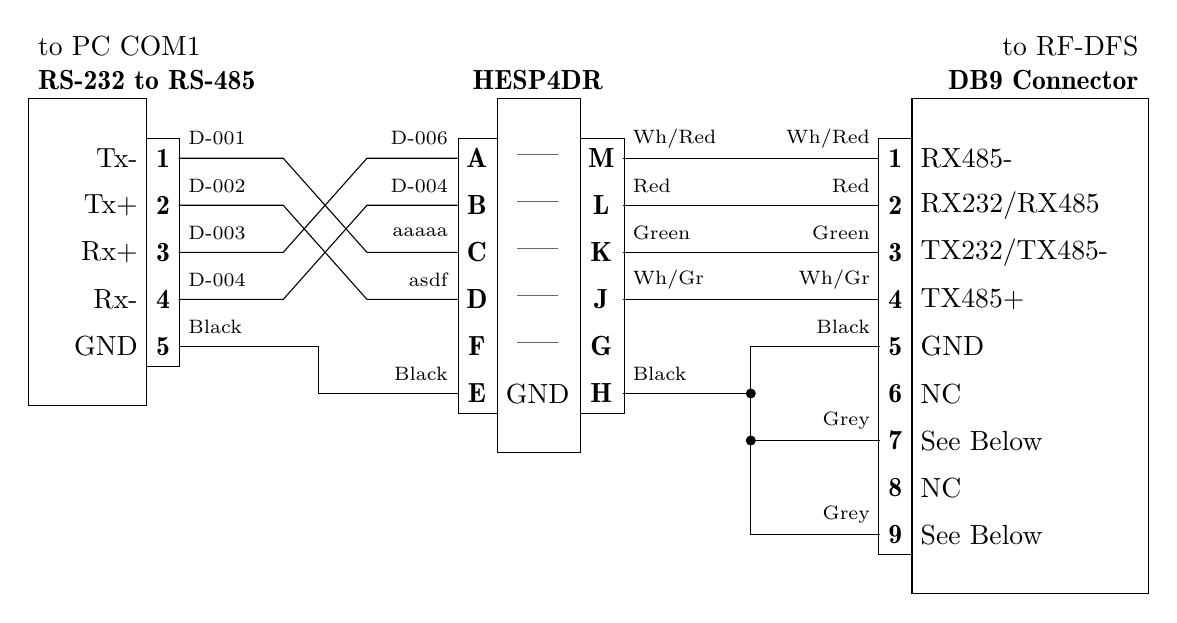
\begin{tikzpicture}
      % \draw[help lines, dashed] grid (12, 3);
      % \draw[help lines, dashed] grid (12, -7);
      % CONVERTER
      \matrix[wire board, wiresright] (converter) {
        Tx-   &  1   &   \scriptsize D-001   \\
        Tx+   &  2   &   \scriptsize D-002   \\
        Rx+   &  3   &   \scriptsize D-003   \\
        Rx-   &  4   &   \scriptsize D-004   \\
        GND   &  5   &   \scriptsize Black   \\
        };
        \draw (converter-1-2.north east) rectangle (converter-5-2.south west);
        \draw (converter-1-2.north west)+(-1.5cm,0.5cm) coordinate(p1) rectangle ($(converter-5-2.south west)+(0,-0.5cm)$);
        \draw (p1) node[anchor=south west, align=left]{to PC COM1\\\textbf{RS-232 to RS-485}};

        % LIGHTNING PROTECTION SYSTEM
        \matrix[wire board, wiresboth, matrix anchor=north, right=5cm of converter.north] (lps) {
          \scriptsize D-006 &   A   &  -----  &  M  & \scriptsize Wh/Red\\
          \scriptsize D-004 &   B   &  -----  &  L  & \scriptsize Red\\
          \scriptsize aaaaa &   C   &  -----  &  K  & \scriptsize Green\\
          \scriptsize asdf  &   D   &  -----  &  J  & \scriptsize Wh/Gr\\
          \scriptsize       &   F   &  -----  &  G  & \scriptsize \\
          \scriptsize Black &   E   &  GND    &  H  & \scriptsize Black\\
        };
        % Boxing the contents
        \draw (lps-1-2.north east) rectangle (lps-6-2.south west);
        \draw (lps-1-4.north east) rectangle (lps-6-4.south west);
        \draw (lps-1-2.north east)+(0cm,0.5cm) rectangle ($(lps-6-4.south west)+(0cm,-0.5cm)$);
        \draw (p1) (current subpath start -| lps-1-3) node[anchor=south, font=\bfseries]{HESP4DR};

        % DB9 CONNECTOR
        \matrix[wire board, wiresleft, matrix anchor=north, right=5cm of lps.north] (db9) {
          \scriptsize Wh/Red &   1   &   RX485- \\
          \scriptsize Red   &   2   &   RX232/RX485 \\
          \scriptsize Green &   3   &   TX232/TX485- \\
          \scriptsize Wh/Gr &   4   &   TX485+ \\
          \scriptsize Black &   5   &   GND  \\
          \scriptsize       &   6   &   NC \\
          \scriptsize Grey  &   7   &   See Below \\
          \scriptsize       &   8   &   NC \\
          \scriptsize Grey  &   9   &   See Below \\
        };
        \draw (db9-1-2.north east) rectangle (db9-9-2.south west);
        \draw (db9-1-2.north east)+(3cm,0.5cm) coordinate(p3) rectangle ($(db9-9-2.south east)+(0,-0.5cm)$);
        \draw (p3) node[anchor=south east, align=right]{to RF-DFS\\\textbf{DB9 Connector}};

        % WIRING this is the most hellish thing i've ever done never make a wiring diagram in tikz it isnt worth it
        \path(converter-1-3.south west) -- (lps-1-1.south east)
        coordinate[pos=0.25](1quarter)
        coordinate[pos=0.375](3eighth)
        coordinate[pos=0.5](m)
        coordinate[pos=0.675](5eighth)
        coordinate[pos=0.75](3quarter);
        
        \draw(converter-1-3.south west) -- (3eighth) -- (lps-3-2 -| 5eighth) -- (lps-3-1.south east);
        \draw(converter-2-3.south west) -- (converter-2-2 -| 3eighth) -- (lps-4-2 -| 5eighth) -- (lps-4-1.south east);
        \draw(converter-3-3.south west) -- (converter-3-2 -| 3eighth) -- (5eighth) -- (lps-1-1.south east);
        \draw(converter-4-3.south west) -- (converter-4-2 -| 3eighth) -- (lps-2-2 -| 5eighth) -- (lps-2-1.south east);
        \draw(converter-5-2) -- (converter-5-2 -| m) |- (lps-6-2);
        
        \draw(lps-1-5.south west) -- (db9-1-2);
        \draw(lps-2-5.south west) -- (db9-2-2);
        \draw(lps-3-5.south west) -- (db9-3-2);
        \draw(lps-4-5.south west) -- (db9-4-2);
        \path(lps-5-5.south west) -- coordinate[midway](m) (db9-5-2);
        \draw(lps-6-5.south west) -- (lps-6-4 -| m) node[circ=1pt](gndm){};
        \draw(gndm) |- (db9-5-1.south east);
        \draw(gndm) -- (db9-7-2 -| gndm) node[circ=1pt](gndm2){} -- (db9-7-1.south east);
        \draw(gndm2) |- (db9-9-1.south east);

\end{tikzpicture}
\end{center}
\caption{RS-485 serial wiring diagram for connecting the PC to the ACR9000 motor controller. Note that Pins 7 and 9 on the ACR9000 should be connected to GND when using 4-wire RS-485 and left open when using RS-232.}\label{fig:serialwiring}
\end{figure}

\begin{figure}[!ht]
  \begin{center}
    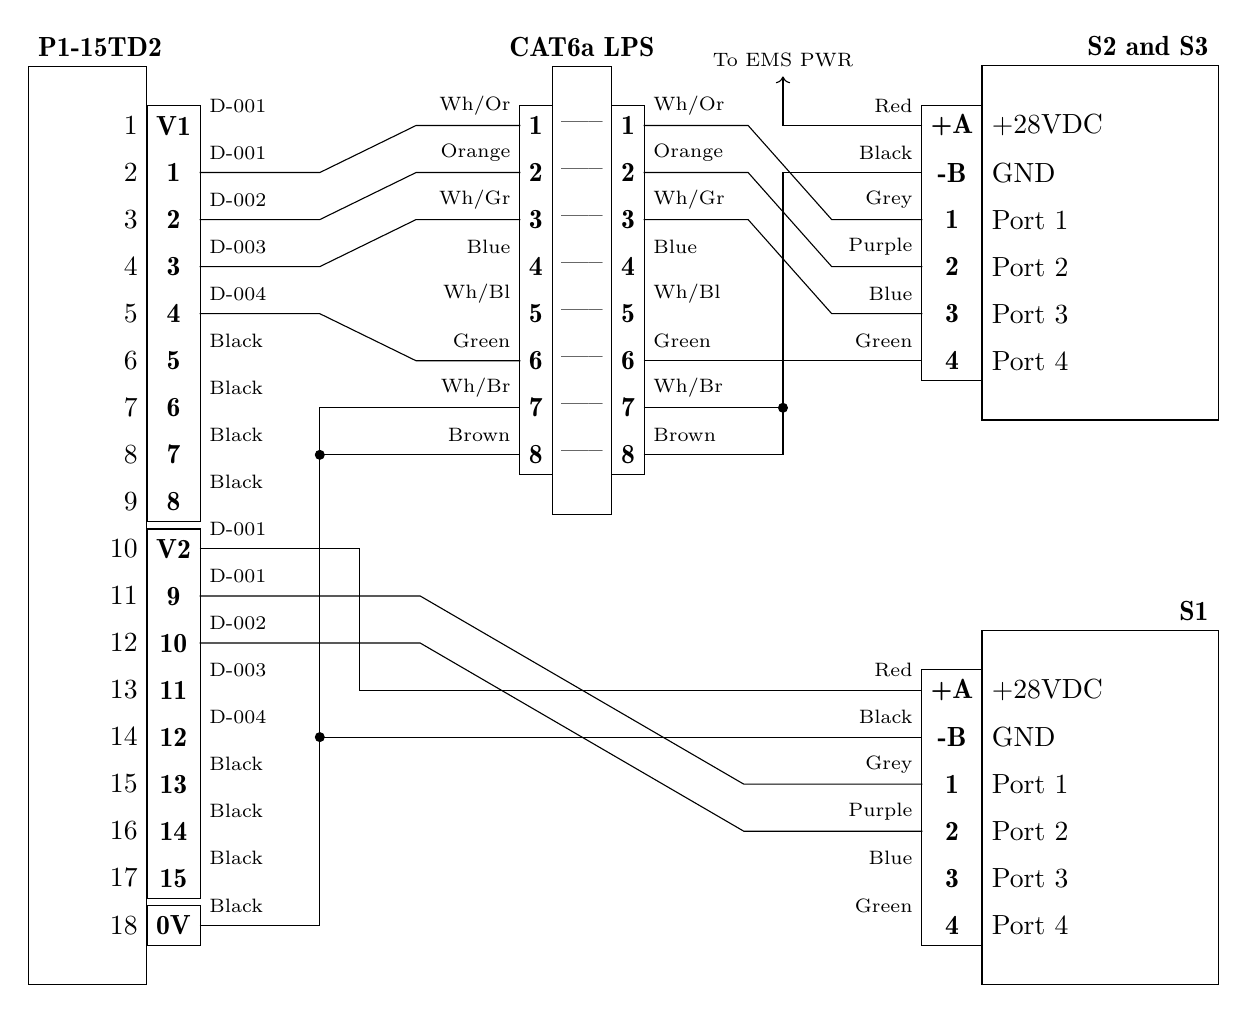
\begin{tikzpicture}
      % \draw[help lines, dashed] grid (12, 3);
      % \draw[help lines, dashed] grid (12, -7);
      % PLC
      \matrix[wire board, wiresright] (plc) {
        1   &  V1  &   \scriptsize D-001   \\
        2   &  1   &   \scriptsize D-001   \\
        3   &  2   &   \scriptsize D-002   \\
        4   &  3   &   \scriptsize D-003   \\
        5   &  4   &   \scriptsize D-004   \\
        6   &  5   &   \scriptsize Black   \\
        7   &  6   &   \scriptsize Black   \\
        8   &  7   &   \scriptsize Black   \\
        9   &  8   &   \scriptsize Black   \\
        10  &  V2  &   \scriptsize D-001   \\
        11  &  9   &   \scriptsize D-001   \\
        12  &  10  &   \scriptsize D-002   \\
        13  &  11  &   \scriptsize D-003   \\
        14  &  12  &   \scriptsize D-004   \\
        15  &  13  &   \scriptsize Black   \\
        16  &  14  &   \scriptsize Black   \\
        17  &  15  &   \scriptsize Black   \\
        18  &  0V  &   \scriptsize Black   \\
        };
        \draw (plc-1-2.north east) rectangle (plc-9-1.south east);
        \draw (plc-10-2.north east) rectangle (plc-17-1.south east);
        \draw (plc-18-2.north east) rectangle (plc-18-1.south east);
        \draw (plc-1-2.north west)+(-1.5cm,0.5cm) coordinate(p1) rectangle ($(plc-18-2.south west)+(0,-0.5cm)$);
        \draw (p1) node[anchor=south west, align=left]{\textbf{P1-15TD2}};

        % CAT6 LIGHTNING PROTECTION SYSTEM
        \matrix[wire board, wiresboth, matrix anchor=north, right=5cm of plc.north] (lps) {
          \scriptsize Wh/Or &   1   &  -----  &  1  & \scriptsize Wh/Or\\
          \scriptsize Orange&   2   &  -----  &  2  & \scriptsize Orange\\
          \scriptsize Wh/Gr &   3   &  -----  &  3  & \scriptsize Wh/Gr\\
          \scriptsize Blue  &   4   &  -----  &  4  & \scriptsize Blue\\
          \scriptsize Wh/Bl &   5   &  -----  &  5  & \scriptsize Wh/Bl\\
          \scriptsize Green &   6   &  -----  &  6  & \scriptsize Green\\
          \scriptsize Wh/Br &   7   &  -----  &  7  & \scriptsize Wh/Br\\
          \scriptsize Brown &   8   &  -----  &  8  & \scriptsize Brown\\
        };
        % Boxing the contents
        \draw (lps-1-2.north east) rectangle (lps-8-2.south west);
        \draw (lps-1-4.north east) rectangle (lps-8-4.south west);
        \draw (lps-1-2.north east)+(0cm,0.5cm) rectangle ($(lps-8-4.south west)+(0cm,-0.5cm)$);
        \draw (p1) (current subpath start -| lps-1-3) node[anchor=south, font=\bfseries]{CAT6a LPS};

        % RF SWITCHES 2 AND 3
        \matrix[wire board, wiresleft, matrix anchor=north, right=5cm of lps.north] (emsswitches) {
          \scriptsize Red   &   +A  & +28VDC \\
          \scriptsize Black &   -B  & GND \\
          \scriptsize Grey  &   1   & Port 1 \\
          \scriptsize Purple&   2   & Port 2 \\
          \scriptsize Blue  &   3   & Port 3 \\
          \scriptsize Green &   4   & Port 4 \\
        };
        \draw (emsswitches-1-2.north west) rectangle (emsswitches-6-3.south west);
        \draw (emsswitches-1-3.north west)+(3cm,0.5cm) coordinate(p3) rectangle ($(emsswitches-6-3.south west)+(0,-0.5cm)$);
        \draw (p3) node[anchor=south east, align=right]{\textbf{S2 and S3}};

        % RF SWITCHES 1
        \path (plc.south) -- (plc.south -| emsswitches.south)
        node[matrix, wire board, wiresleft, matrix anchor=south] (shackswitch) {
          \scriptsize Red   &   +A  & +28VDC \\
          \scriptsize Black &   -B  & GND \\
          \scriptsize Grey  &   1   & Port 1 \\
          \scriptsize Purple&   2   & Port 2 \\
          \scriptsize Blue  &   3   & Port 3 \\
          \scriptsize Green &   4   & Port 4 \\
        };
        \draw (shackswitch-1-2.north west) rectangle (shackswitch-6-3.south west);
        \draw (shackswitch-1-3.north west)+(3cm,0.5cm) coordinate(p3) rectangle ($(shackswitch-6-3.south west)+(0,-0.5cm)$);
        \draw (p3) node[anchor=south east, align=right]{\textbf{S1}};

        % WIRING 
        % plc to lps
        \path(plc-1-3.south west) -- (lps-1-1.south east)
        coordinate[pos=0.25](1q)
        coordinate[pos=0.375](3e)
        coordinate[pos=0.5](m)
        coordinate[pos=0.675](5e)
        coordinate[pos=0.75](3q);
        \draw(plc-2-3.south west) -- (plc-2-1 -| 3e) -- (lps-1-2 -| 5e) -- (lps-1-1.south east);
        \draw(plc-3-3.south west) -- (plc-3-1 -| 3e) -- (lps-2-2 -| 5e) -- (lps-2-1.south east);
        \draw(plc-4-3.south west) -- (plc-4-1 -| 3e) -- (lps-3-2 -| 5e) -- (lps-3-1.south east);
        \draw(plc-5-3.south west) -- (plc-5-1 -| 3e) -- (lps-6-2 -| 5e) -- (lps-6-1.south east);
        % plc to shack switch
        \draw(plc-10-3.south west) -- (plc-10-3.south west -| m) -- (shackswitch-1-1.south east -| m) -- (shackswitch-1-1.south east);
        \draw(plc-11-3.south west) -- (plc-11-3.south west -| lps.west) -- (shackswitch-3-1.south east -| lps.east) -- (shackswitch-3-1.south east);
        \draw(plc-12-3.south west) -- (plc-12-3.south west -| lps.west) -- (shackswitch-4-1.south east -| lps.east) -- (shackswitch-4-1.south east);
        % plc ground wires
        \draw(plc-18-3.south west) -- (plc-18-3.south west -| 3e) -- (shackswitch-2-1.south east -| 3e) node[circ=1pt](gndnode1){};
        \draw(gndnode1) -- (shackswitch-2-1.south east);
        \draw(gndnode1) -- (lps-8-1.south east -| gndnode1) node[circ=1pt](gndnode2){} -- (lps-8-1.south east);
        \draw(gndnode2) |- (lps-7-1.south east);
        % lps to ems switches
        \path(lps-1-5.south west) -- (emsswitches-1-1.south east)
        coordinate[pos=0.25](1q)
        coordinate[pos=0.375](3e)
        coordinate[pos=0.5](m)
        coordinate[pos=0.675](5e)
        coordinate[pos=0.75](3q);
        \draw(lps-1-5.south west) -- (lps-1-5.south west -| 3e) -- (emsswitches-3-2 -| 5e) -- (emsswitches-3-1.south east);
        \draw(lps-2-5.south west) -- (lps-2-5.south west -| 3e) -- (emsswitches-4-2 -| 5e) -- (emsswitches-4-1.south east);
        \draw(lps-3-5.south west) -- (lps-3-5.south west -| 3e) -- (emsswitches-5-2 -| 5e) -- (emsswitches-5-1.south east);
        \draw(lps-6-5.south west) -- (emsswitches-6-1.south east);
        \draw(lps-8-5.south west) -- (lps-8-5.south west -| m) -- (emsswitches-2-1.south east -| m) -- (emsswitches-2-1.south east);
        \draw(lps-7-5.south west) -- (lps-7-5.south west -| m) node[circ=1pt]{};
        \draw(emsswitches-1-1.south east)[->] -- (m) -- (m |- emsswitches.north) node[anchor=south]{\scriptsize To EMS PWR};
        
\end{tikzpicture}
\end{center}
\caption{AAAAAAAAAAAAAAHHHHHHHHHHHHHHHHHH.}\label{fig:rfswitchwiring}
\end{figure}

\subsection{RF-DFS Components}
motor controller, motors, serial lps
\subsection{RF-EMS Components}
switching, amplifiers, lps,

\section{Communications}
maybe put pinouts and connections here instead to keep them all together
\subsection{Spectrum Analyzer}
scpi commands, how it works, etc, explain not to issue commands while program is running
\subsection{Motor Controller}
aries command reference stuff here, what bits are used
\subsection{PLC}
opcodes

\section{Software User Guide}
copy everything from github wiki
\subsection{Getting Started}
software installation stuff, ni-visa, other requirements

In order to use the front-end interface, download the following deployment requirements and the latest release on \verb|EMSMONPC2|, then run the executable.
\begin{enumerate}
  \item NI-VISA
  \item NI-488.2 if the spectrum analyzer connection is GPIB
\end{enumerate}

\subsection{Using the Program}
After starting the program, navigate to \verb|Options>Configure| at the top left banner to connect to the appropriate devices/COM ports. The \verb|Connection Status| window will let you know if a device is connected, however, it is up to the user to ensure that the correct device has been selected in the \verb|Configure| menu. The terminal will output any initialization errors (such as if the wrong device/port is selected).

From here, the user can issue SCPI commands to the spectrum analyzer using the control panel on the right, issue motor commands using the \verb|Antenna Position| panel, or select RF chains using the \verb|PLC Operations| panel on the left. Commands can be issued to the spectrum analyzer by either selecting a button or typing an entry and pressing \verb|Enter|. All entries will be issued in base units for the given parameter (Hz, seconds, etc.), however, shorthand scientific notation is allowed (5e9 will be passed as 5 GHz).

\begin{figure}
  \begin{center}
    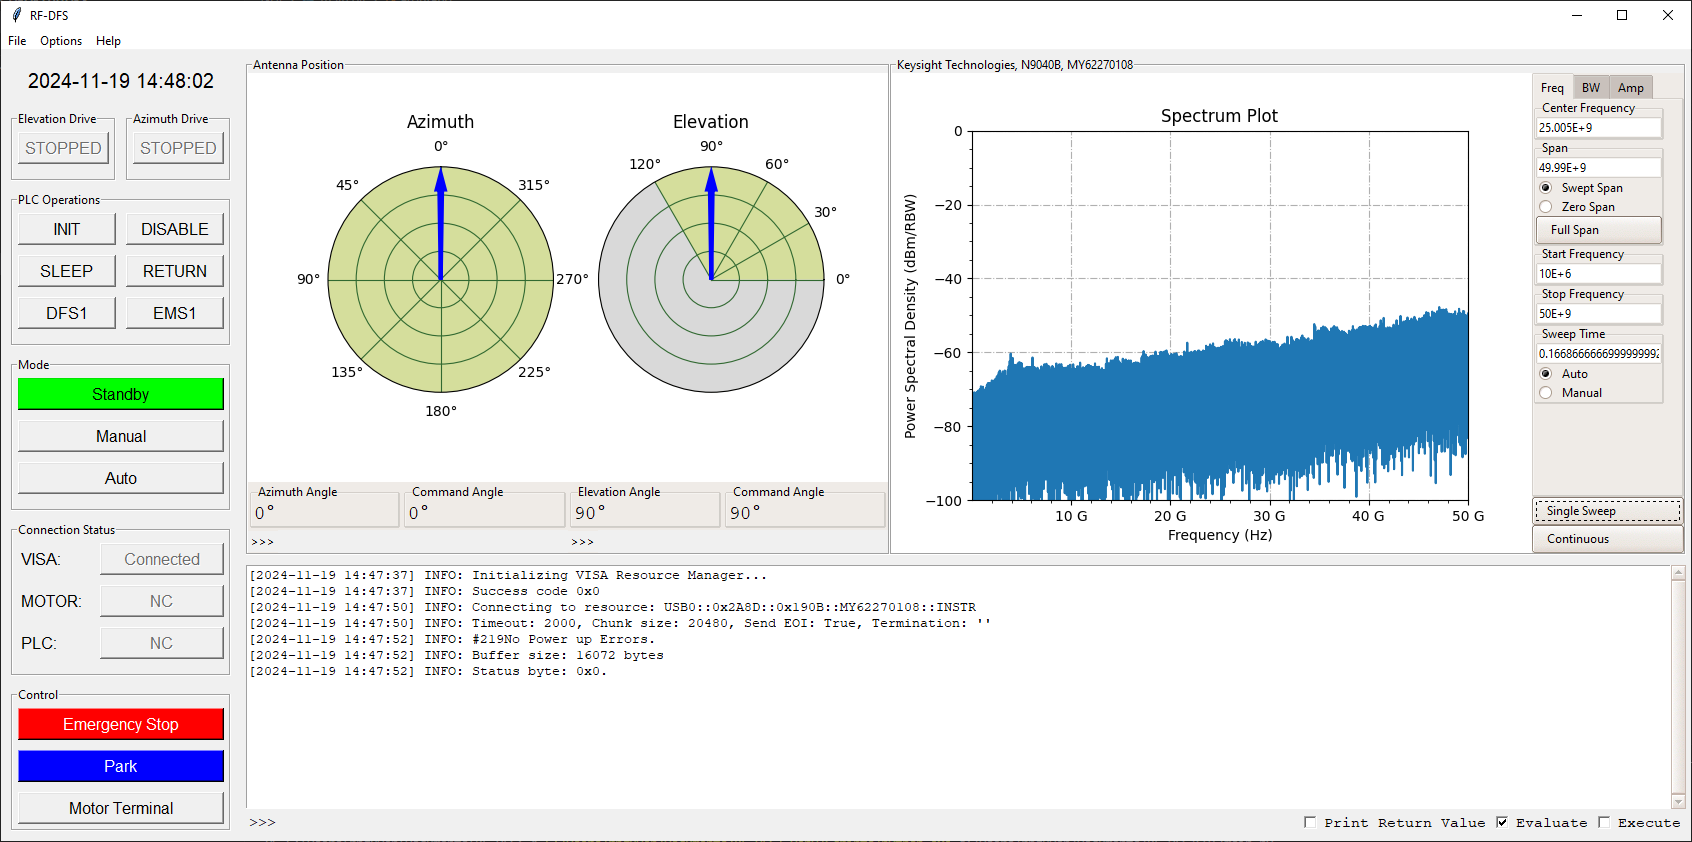
\includegraphics[width=\textwidth]{images/3gui.png}
  \end{center}
  \caption{asdf}\label{fig:gui}
\end{figure}

\subsubsection{Header}
\subsubsection{Control Panel}
\subsubsection{Antenna Position}
\subsubsection{Spectrum Analyzer Controls}
\subsubsection{Terminal}
Python commands can also be evaluated or executed in the terminal, the difference between both commands is described in the Python documentation. It is highly recommended to reference the source code when issuing terminal commands, as this has the potential for deadlock, race conditions, and other undefined scenarios if care is not taken. Instances, their attributes, and methods, can all be accessed using the terminal although all commands will be generated in the main thread. As a result, most IO calls will be blocking for the duration of their execution. This can be avoided by using a thread handler, if it exists in the appropriate scope, or generating a thread for the given IO call. See:

\verb|SpecAn.setAnalyzerThreadHandler|:
\begin{lstlisting}[language=Python]
class SpecAn(FrontEnd):
    def setAnalyzerThreadHandler(self, *event, **kwargs):
        _dict = {}
        for key in kwargs:
            _dict[key] = kwargs.get(key)
        thread = threading.Thread(target=self.setAnalyzerValue, kwargs=_dict)
        thread.start()
\end{lstlisting}

\verb|SerialIO.threadHandler|:
\begin{lstlisting}[language=Python]
class SerialIO:
    def threadHandler(self, target, args=(), kwargs={}):
        if not hasattr(SerialIO, target.__name__):
            logging.error(f'Class SerialIO does not contain a method with identifier {target.__name__}')
            return
        thread = threading.Thread(target = target, args = args, kwargs = kwargs, daemon=True)
        thread.start()
\end{lstlisting}

Or, if generating a thread using the \verb|Execute| function, use semicolons to separate lines of code.
\begin{lstlisting}[language=Python]
thread=threading.Thread(target=Vi.openRsrc.write, args=(":SENS:FREQ:STOP 10e9",), daemon=True);thread.start()
\end{lstlisting}
Is equivalent to\dots
\begin{lstlisting}[language=Python]
thread=threading.Thread(target=Vi.openRsrc.write, args=(":SENS:FREQ:STOP 10e9",), daemon=True)
thread.start()
\end{lstlisting}  

\end{document}


